\documentclass[oneside,a4paper,titlepage]{article}
\usepackage{blindtext}
\usepackage[utf8]{inputenc}
\usepackage{verbatim} 
\usepackage{graphicx}
\usepackage{color}
\usepackage{float}
\usepackage[hidelinks]{hyperref}
\usepackage{lipsum}
\usepackage{pdfpages}
\usepackage{geometry}
\usepackage[font={small,it}]{caption}
\usepackage{booktabs}
\usepackage{amsmath}
\usepackage{amssymb}
\usepackage{listings}
\usepackage{tikz}
\usepackage{tikz-3dplot}
\usetikzlibrary{arrows.meta}
\usetikzlibrary{trees}
\usepackage{courier}
\usepackage{esvect}
\usepackage{subcaption}

 \geometry{
 % a4paper,
 % total={170mm,217mm},
 % left=20mm,
 % top=40mm,
 }
% \oddsidemargin=-10pt
% \textwidth=450pt
% \textheight=5cm0
\setlength\parindent{0pt} % sets indent to zero
\setlength{\parskip}{6pt} % changes vertical space between paragraphs
\renewcommand{\baselinestretch}{1.2} % sets lineheight

% Mappe hvori billeder ligger
\graphicspath{ {graphics/} }

% Tekst som står først i figur captions "{Figure/Figur} 3: Pixelering der fremkommer..."
\renewcommand{\figurename}{Figur}
\renewcommand{\abstractname}{Abstrakt}
\renewcommand\refname{}

\definecolor{codegreen}{rgb}{0,0.6,0}
\definecolor{codegray}{rgb}{0.5,0.5,0.5}
\definecolor{codepurple}{rgb}{0.58,0,0.82}
\definecolor{backcolour}{rgb}{0.95,0.95,0.92}
 
\lstdefinestyle{Cstyle}{
    %backgroundcolor=\color{backcolour},
    language=C,   
    commentstyle=\color{codegreen},
    keywordstyle=\color{blue},
    numberstyle=\color{codegray},
    stringstyle=\color{codepurple},
    basicstyle=\footnotesize,
    breakatwhitespace=false,         
    breaklines=true,                 
    captionpos=b,                    
    keepspaces=true,                 
    numbers=left,                    
    numbersep=5pt,                  
    showspaces=false,                
    showstringspaces=false,
    showtabs=false,     
    basicstyle=\ttfamily,breaklines=true,           
    morekeywords={Vector, Pixel, Ray, Image, PointLight, FILE, Triangle, Vertex, Material, Object, Camera},  
    tabsize=2
}




% supresses errors during compilation
% \batchmode

%\title{Ray Tracing}
%\author{P1 B2-28}
%\date{\today}

\begin{document}
%\maketitle

% \begin{abstract}
% Abstract text placeholder, lorem ipsum dolor sit amet...
% \end{abstract}


% sections
\begin{titlepage}
  %\toprule[2pt]
  %\midrule
  \vspace{0.2cm}
  \begin{center}
    \Huge{\textbf{Visualisering af lampers belysning}}
  \end{center}
  \vspace{0.2cm}
  %\midrule
  %\toprule{2pt}
  \begin{center}
    \Large{\textbf{Gruppe B2-28}}\\
	Morten Rask Andersen\\
	Christian Mønsted Grünberg\\
	Anton Christensen\\
	Mathias Ibsen\\
	Lasse Fribo Gadegaard\\
	Mathias Rohde Pihl
  \end{center}
  \vfill
  \begin{center}
 	\today\\
    Aalborg Universitet\\
    Software, 1. semester
  \end{center}
\end{titlepage}

%Synopsis

\thispagestyle{empty}
\noindent\begin{tabular}{ll}

\includegraphics[height=1.5cm]{awesome} & 
\includegraphics[height=1.5cm]{a} \\
\makebox[2.5in]{\hrulefill} & \makebox[2.5in]{\hrulefill}\\
Morten Rask Andersen & Anton Christensen\\[8ex]

\includegraphics[height=1.2cm]{las} & 
\includegraphics[height=1.2cm]{chr} \\
\makebox[2.5in]{\hrulefill} & \makebox[2.5in]{\hrulefill}\\
Lasse Fribo Gadegaard & Christian Grünberg\\[8ex]

\includegraphics[height=1.5cm]{ibbe} & 
\includegraphics[height=1.4cm]{pihl} \\
\makebox[2.5in]{\hrulefill} & \makebox[2.5in]{\hrulefill}\\
Mathias Ibsen & Mathias Pihl\\[8ex]
\end{tabular}

\clearpage

\section{Forord}
Denne rapport er udarbejdet af gruppe B2-28, bestående af software-studerende, som P1-rapport på Aalborg Universitet.

Rapporten tager udgangspunkt i Aalborg-modellen for problembaseret læring. Denne læringsproces har givet gruppen mulighed for at undersøge en given problemstilling og derudfra tilegne sig viden, og på baggrund af denne viden udarbejde en problemanalyse. Derudover gør rapporten brug af den kvalitative metode til korrespondance med interessenterne. Den kvalitative metode er fordelagtig at bruge, når man vil undersøge forhold, som er svære at iagttage eller måle \cite{kvalitativ_metode}. Problemanalysen har herefter, gennem et samarbejde med erhvervslivet, hjulpet med at afgrænse og danne fundamentet for problemløsningen. I forbindelse med samarbejdet med erhvervslivet har vi taget kontakt til en række lampebutikker. Disse butikker og deres kommentarer vil efter eget ønske fremgå anonymt. 

Tak til vejledere Benjamin Bjerre Krogh og Annette Grunwald samt de medvirkende belysningskonsulenter, designere og lampebutikker.
\clearpage
\subsection{Læsevejledning}
Rapporten er skrevet med en rød tråd, hvilket vil sige, at afsnittene er struktureret således, at der gerne skulle skabes en sammenhæng mellem afsnittene og herefter en helhed. Det er dog ikke nødvendigt at læse hele rapporten, da hvert afsnit har sin egen indledning og opsummering hhv. først og sidst i afsnittet.

Programmet er uploadet til Digital Eksamen og er derfor elektronisk bilag. 

\subsubsection{Kildehenvisning}
Rapportens brug af kildehenvisninger er baseret på nummermetoden \cite{nummermetoden}. I nummermetoden anføres kilderne i fortløbende nummerorden, svarende til hvilket nummer, de har i teksten. To identiske kilder har samme nummer. Herunder ses et eksempel på henvisninger til hhv.\ internetkilder, artikler og bøger:

Interneteksempel med kilde[1].

[1] Titel på emne eller kort forklaring på emnet, hjemmesidenavn. Set DD-MM-YYYY. URL på hjemmeside.


Bogeksempel med kilde[2].

[2] Titel på bog, udgavenummer, forfatter(e), udgivelsesår. ISBN/ISSN-nummer.


Hvis en kilde har yderligere relevante informationer (såsom sidetal, ophavsret mm.\ angives disse også i kilden.


Figurhenvisning foregår på samme måde som med andre kilder, dog med en forklaring under selve figuren. Hvis en figur ingen kilde har, er figuren fremstillet af gruppen.


\subsubsection{Kodeuddrag}
Flere steder i rapporten, vil der blive vist dele af gruppens kode. Et eksempel på hvordan dette vil blive vist er herunder:

\begin{lstlisting}[style=Cstyle, caption=Kodeeksempel i C]
#include <stdio.h>

int main(void){
   printf("Hello, world!\n");
   return 0;
}
\end{lstlisting}

\clearpage

\tableofcontents
\clearpage

Selvom vi ikke tænker på det så ofte, så er lamper en stor del af vores hverdag. De står i vores hjem, på vores gader, på vores arbejdsplads - ja de er stort set overalt. Men hvorfor er lamper egentlig så udbredte? Det er de, fordi lamper bliver brugt til at skabe lys. Belysning kan bidrage til mange ting som at læse, arbejde mere koncentret eller til at skabe hygge og stemning i et rum, der ellers ville have været koldt og kedeligt. 
\newline Lamper findes i mange forskellige typer og mange forskellige steder. Der er læselamper, arbejdslamper, loftlamper, udendørslamper osv. og de tjener allesammen forskellige formål, men fælles for dem er, at de skaber lys steder hvor der ellers ikke ville have været lys. 
I dag findes der utroligt mange forskellige lampedesigns, og de er ikke allesammen lige gode. Dette vil sige at nogle lamper har meget dårlig belysning. Dette er et problem, da undersøgelser har vist at dårlig belysning kan føre til blandt andet øjenskader, hovedpine samt ondt i nakke og hals \cite{lys_konsekvenser}. Andre problemer kan også opstå, hvis en lampe har en for kraftig belysning, og derfor er blændende eller hvis f.eks en udendørs lampe ikke lyser tilstrækkeligt, og man derfor vælter, fordi man ikke kan se noget. 
Så selvom lamper spiller en stor rolle i vores hverdag, så er det vigtigt at kunne visualisere hvordan lys udbreder sig fra en lampe, så man kan undgå dårlig belysning. 
\newline Man kan derfor argumentere for at det essentielle ved en lampe ikke er dens design, men er det lys som den udsender, herunder mønster og farve, samt lysets indflydelse på indretning og belysning. Med afsæt i denne argumentation har vi derfor valgt at arbejde med visualisering af lyset fra lamper.

\subsection{Motivation}

Som studerende på software synes vi, at det kunne være interresant at arbejde med et håndterbart problem som der ville kunne findes en teknologisk løsning på. 
\newline Gruppens mål er derfor at finde et relevant problem indenfor visualisering af lyset fra lamper, og derudfra lave en teknologisk løsning på problemet. Som gruppe er vi motiveret af, at vi kan designe og implementere software med henblik på at finde en god løsning på et relevant problem. 

\subsection{Initierende problem}

I indledningen slog vi som gruppe fast, at vi gerne ville arbejde med visualisering af lyset fra lamper. På baggrund af vores viden om lys fra lamper, samt de erfaringer og diskussioner vi har foretaget os som gruppe, har vi valgt at opstille følgende initierende problem:

Forbrugeren kan ikke visualisere, hvordan lyset udbreder sig fra en lampe uden at købe og installere lampen.

\section{Problemanalyse}
\subsection{Begrebsligørelse}
Der er indtil videre blevet  argumenteret for relevansen af det initierende problem, og det er i den sammenhæng derfor nødvendigt at redegøre for nogle vigtige emner og ord indenfor problemfeltet. 

Formålet med dette afsnit er at beskrive vigtige begreber samt kort at give en beskrivelse af, hvordan de forskellige ord og begreber skal forstås i den videre rapport. Begreberne som fremgår i følgende afsnit danner grundlag for forståelsen af det initierende problem. Disse begreber er følgende: Forbruger, visualisering, lys og lamper.

% \subsubsection{Køber}
% En køber er en person, der køber et produkt eller tjenesteydelser \cite{ddo_forbruger}.  Køberen står altså i denne sammenhæng i modsætning til producenterne.
% I denne rapport opfattes køberen som den person der køber lampen. Det vil altså sige, at der i dette tilfælde ikke nødvendigvis er tale om personer der til dagligt bruger eller bliver påvirket af lampen.

\subsubsection{Forbruger}
En forbruger er en privatperson som køber et produkt eller tjenesteydelser. “Forbruge” betyder at “bruge noget”, og en forbruger køber derfor produkter med henblik på at tilfredsstille nogle behov \cite{forbrugerportalen}. En bevidst forbruger, vil derfor ofte lede efter produkter der opfylder deres behov. Man antages også for at være forbruger af en varer hvis man til daglig benytter sig af eller bliver påvirket af en given lampe. 

I vores rapport udvider vi definitionen af forbruger til, at en forbruger også kan være en erhvervsperson der køber en lampe til brug i virksomheden. Derudover hører en kunde også til under begrebet forbruger, da det er kunderne som køber lamperne. 

%\subsubsection{Sælger}
%En sælger er den person eller virksomhed der sælger et produkt eller %tjenesteydelser. I rapporten opfattes sælgeren som værende en person %eller virksomhed, der sælger lamper til forbrugeren. 

\subsubsection{Visualisering}
At visualisere, betyder at skabe et billede på baggrund af noget \cite{ddo_visualisering}. Dette kan til dels være tanker, som omsættes til billeder for det indre øje. Det kan også være en række data, som omsættes til billeder, så de er nemmere at forstå.
Visualisering kan være et redskab til at skabe en forståelse for det der visualiseres. Dette kan f.eks være prototyper af lamper, der kan give en forståelse for hvordan lyset udbreder sig fra en lampe. Derudover er der inden for computergrafik metoder til at skabe billeder på baggrund af 3D-modeller, så man f.eks. kan lave et delvist realistisk billede af en lampe, og på den måde få en forståelse for hvordan lampen ser ud i virkeligheden og hvordan dens lys udbredes. Forskellige teknologier til visualisering er uddybet senere i rapporten under afsnit \ref{sec:teknologianalyse}. 

\subsubsection{Lys}
Der er forskellige opfattelser af hvad lys det indebærer. Hvis vi tager udgangspunkt i Karsten Rottwitt, som er professor ved DTU fotonik, så påstår han at lys er:

“Lys er andet end synligt lys. For mig er lys et elektromagnetisk felt, som har en høj frekvens”
- Karsten Rottwitt\cite{def_lys}.

Han mener også, at der er en hårdfin grænse for hvornår lys kan betegnes som lys, denne grænse er dog først i spil når vi snakker om UV-lys og infrarødt lys \cite{def_lys}. 
Andre er ikke enige med Karsten Rottwitt om hvordan definitionen af lys er. Tager vi nu udgangspunkt i Britannica \cite{britannica_lys}, så betegnes lys, som magnetiske stråler, som det menneskelige øje kan opfange - Hvilket vil sige, lys med en bølgelængde mellem 380 og 750 nanometer, også kaldet synligt lys. 

Det er denne definition, som rapporten vil tage udgangspunkt i. Dette er valgt, da det er oplagt at kombinere synligt lys og lamper \cite{def_lys}.

Det lys som kommer fra en lampe, er selvfølgelig af forskellig kvalitet. Kvalitet kan ligesom lys, betegnes på mange måder, herunder kan vi snakke om hvorvidt en lyskilde er af god kvalitet, hvis den er energivenlig eller om det kun kommer an på hvor gode de er til at eftergive farvet lys. 
Afhængigt af hvor man skal bruge lyset, kan nogle former for lys være bedre egnet end andre. Her menes der om hvorvidt lyset skal være varmt eller koldt. Integral-led er et firma med over 25 års erfaring\cite{integral_led}, og har opstillet nogle foretrukne steder at bruge de forskellige typer af lys:

Varm / varm hvid = Stue, soveværelse eller gange.
Hvid / kold hvid = Køkken, studie, badeværelser, skrivebord, kontor eller butikker\cite{varm_kold}.

Ud fra disse foretrukne placeringer, opstillet af integral-led, kan vi antage at lys kvaliteten blandt andet afhænger af hvor lyset skal bruges. Hvis det er i et stille og roligt miljø, med henblik på at slappe af, er det måske at foretrække det varme lys, hvormid de steder hvor det er nødvendigt at have skarpt lys, for evt. at kunne se detaljer eller koncentrere sig, er det kolde lys at foretrække.

\subsubsection{Pærer}
I denne rapport forstås en pærer, som en enhed der ved hjælp af elektricitet udsender lys. Herunder er der forskellige typer pærer, men hvilken skal man vælge? Sparepærer, LED eller halogen?
Da der findes så mange pærer, er der visse ting, der er værd at overveje. En pærer har en Ra-værdi, som bruges til at bedømme hvor god en farvegengivelse pæren har. Ra-skalaen går helt op til 100, hvor det kun er sollys som har en Ra-værdi på 100, der er dog nogle typer af pærer, som næsten kan ramme de 100 Ra.\cite{halogen_paere}

En anden overvejelse er hvor energivenlig pæren skal være, da det svinger meget afhængigt af hvilken pærer der bruges. Ser man på nogle af fordelene ved LED pærer, så er de billige i drift da de har en lang levetid, på ca. 25 år, samt et lavt energiforbrug\cite{LED}, 4-5 gange så lidt, i forhold til halogenpæren, som kun har en levetid på ca. 2år\cite{vaelg_paere}. 
Der findes pærer, som eftergiver bedre end andre, og blandt toppen findes Halogen pæren, som kan komme op på 99 Ra, hvilket næsten giver perfekt lys\cite{halogen_paere}. 

Fælles for alle typer af pærer, kan kvaliteten svinge afhængig af hvilken producent. Men hvilken pærer der er bedst, er svært at sige. De har alle sine fordele og ulemper, men går man efter levetid er LED pæren bedst, samt der er mange penge at spare i løbet af de år. Halogen pæren er rigtig god til at eftergive farve, da den har en kelvin på ca. 2500-3000, samt en høj Ra-værdi. Er det en god grundbelysning, samt rimelig billig i indkøb samt drift, så er sparepæren en god løsning, undtagen hvis det er til udendørs brug, da pæren mister lys og levetid ved -20 grader\cite{sparepaerer}.

Det kan konkluderes udfra ovenstående, at kvaliteten af en lyskilde, afhænger af hvor lyset skal bruges, for de forskellige pærer er alle gode, afhængigt af hvor den placeres. Udover kvaliteten af pæren, kan det antages at de forskellige pærer afgiver lys på forskellige måder og dermed kan det være svært at forudse hvordan lampen og lyset kommer til at se ud.  


\subsubsection{Lamper}
Formålet med dette afsnit er at afgrænse definitionen af hvad en lampe er i vores kontekst og hvordan begrebet skal forstås i rapporten.
Der findes mange forskellige definitioner på hvad en lampe faktisk er, og det viser sig ifølge American Heritage® Dictionary of the English Language \cite{american_heritage}, at begrebet ’lampe’ faktisk dækker over mange forskellige ting. 

American Heritage definerer en lampe som værende én eller flere af følgende:

En af flere forskellige enheder, der genererer lys og ofte varme, især:
\begin{enumerate}
    \item En elektrisk anordning, der har en sokkel til en pære, især et fritstående stykke møbel.
    \item En anordning, der afgiver ultravoilet, infrarød, eller anden stråling, som kan anvendes til terapeutiske formål.
    \item En pære: en projektør/et spot(light), udstyret med metalhalogenlampe.
    \item En lanterne eller armatur, der afgiver lys ved afbrænding af gas, ofte ved brug af en kappe.
\end{enumerate}

Idet der er så mange forskellige definitioner på en lampe, er vi, i konteksten af vores projekt, nødsaget til at afgrænse begrebet til noget mere specifikt. Da vi vil hjælpe forbrugeren, med at visualisere lampen i et givet rum, tager vi udgangspunkt i en mere normal lampe. Hvis man kigger på de tidligere definitioner af en lampe, kan man forestille sig utroligt mange apparaturer, som kan kaldes for en lampe. Lige fra ultraviolette lamper, der bruges i natklubber med fluoserende formål, til infrarøde lamper, der kan bruges i medicinske/terapeutiske sammenhænge, fx til at løsne og afspænde musklerne \cite{lys_terapi}. Der findes også lamper, der afgiver lys og varme ved afbrænding af fx gas, såsom en lanterne. For at afgrænse alle disse definitioner, vil en lampe i det videre arbejde med rapporten opfattes som en indendørs anordning, hvori der kan isættes en pære, som kan udsende lys, der evt. afskærmes af anordningen.

\paragraph{Opsummering}
Ud fra de ovenstående afsnit i begrebsliggørelsen, kan der nu kortfattes at der senere i denne rapport anvendes de omtalte begreber med følgende betydning:
\begin{enumerate}
	\item Forbruger: En person der køber en lampe med henblik på brug i hjemmet eller i en virksomhed.
	%\item Sælger: En person eller virksomhed der sælger produkter.
	\item Visualisering: Skabelsen af et billede på baggrund af noget, der evt. ønskes lettere forståeligt.
	\item Lys: Den elektromagnetiske stråling der er synligt for øjet (Synligt lys).
	\item Pære: En enhed der ved hjælp af elektricitet udsender lys.
	\item Lampe: En indendørs anordning hvor der kan isættes en pære, som udsender lys der evt. afskærmes af anordningen.
\end{enumerate}
Ud fra de ovenstående begreber, skulle der nu være en entydig forståelse af det initierende problemet, som gør at problemet nu kan analyseres videre i de kommende afsnit.






\subsection{e-handel}
e-handel er elektronisk handel via internettet. På internettet kan sælgere inden for e-handel have såkaldte e-butikker, hvor kunder kan købe varer. E-butikker er ofte udformet således at kunden kan se billeder og informationer omkring sælgerens varer og derudfra kan kunden vælge at lægge varerne i en virtuel indkøbskurv, hvor kunden til sidst indtaster de nødvendige oplysninger for at købe og modtage varerne.
%http://ordnet.dk/ddo/ordbog?query=ebutik
%http://ordnet.dk/ddo/ordbog?query=ehandel


Blandt de mange forskellige varer, der sælges via e-butikker, er det her relevant at tale om e-handel med lamper. Nedenstående figur \ref{e_handel_med_lamper} illustrerer princippet bag en lampesælgers salg af lampe til en kunde via en e-butik.
\begin{figure}[H]
	\centering
	\def\svgwidth{\columnwidth}
	\input{./e_handel_med_lampe.pdf_tex}
	\caption{Princippet bag handel af en lampe via en e-butik.}\label{e_handel_med_lamper}
\end{figure}

På figur \ref{e_handel_med_lamper} er det vist hvordan e-handlen starter med at kunden får et udvalg af lamper fra e-butikken. Kunden sender så en bestilling, som via e-butikken sendes videre til lampesælgeren, og til sidst sendes lampen til kunden. Dog ender handlen ikke nødvendigvis her, da kunden kan sende lampen retur såfremt at gældende lovgivning og købsbetingelser muliggører dette. For at undersøge lovgivningen nærmere kan man tage udgangspunkt i den danske lov om forbrugeraftaler.
%https://www.retsinformation.dk/forms/r0710.aspx?id=160666#Kap4

I lovens kapitel 1, § 1, stk. 2, nr. 1, fremgår der at lovens bestemmelser for fortrydelsesret gælder for aftaler, som er indgået ved fjernsalg. For en  fjernsalgsaftale gælder der, at aftalen om varer, er indgået gennem fjernkommunikation, hvor den erhvervsdrivende og forbrugeren ikke mødes fysisk (jf. kap. 1, § 3, nr. 1).

Ser man nu på loven i forbindelse med e-handel, foregår fjernkommunikationen gennem internettet via e-butikken, hvor fjernsalgsaftalen udføres i form af brugerens bestilling af f.eks. en lampe. Dette gør at fortrydelsesretten gælder ved e-handel.

Fortrydelsesretten er en forbrugers mulighed for at melde sig ud af en aftale, herunder køb af lamper ved e-handel. Hvis en en forbruger eksempelvis køber en lampe via en e-butik, har forbrugeren mulighed for at fortryde købet inden 14 dage ved at meddele dette til den erhvervsdrievende (jf. kap. 4, § 19). Herefter har forbrugeren 14 dage til at returnere varen (jf. kap. 4, § 24). Hvis varens værdi er forringet som følge af forbrugeren unødvendige håndtering af varen for at inspicere denne, så hæfter forbrugeren for denne værdiforringelse (jf. kap. 4, § 24, stk. 5). Dvs. at hvis en bruger installerer og bruger lampen, hvor der f.eks. tilpasses ledninger, så kan lampens værdi forringes og forbrugeren skal hæfte for dette. 








\subsection{Teknologianalyse}

Vi ser en tydelig mulighed for at assistere forbrugere med at træffe et valg når det kommer til (køb af vare på nettet | bestemmelse af optimale lysforhold i hjemmet | visualisering af et tilkøbt element i forbrugernes dagligdag/hjem). Dette vil sandsynligvis kunne løses ved hjælp af bedre købsvejledning eller værktøjer til at assistere forbrugeren i en købssituation hvor en prøve ikke kan stilles til rådighed eller at returnere varen er umuligt eller for omfattende en process.

% // redegørelse
Blot at vælge en lampe fra et katalog er problematisk hvis der ikke er billeder af lampen som 
\begin{enumerate}
    \item Fremviser lampen som møbel, rent visuelt, det fysiske design og 
    \item Viser hvordan lys kastes af lampen. En god løsning vil være at have en fysisk model placeret i en kontekst hvor man kan komme og se lampen og se lyset i sammenspil med anden indretning, sålledes som f.eks. Ikea gør.
\end{enumerate}
\begin{figure}[H]
    \centering
    \fbox{\rule{\textwidth}{5cm}}
    \caption{Ikea hus billede}
    % https://www.pinterest.com/pin/6685099420243693/
\end{figure} 

Man vil også kunne skabe billige prototyper af lamper vha. 3D printer tekniker. Disse ville eventuelt være mulige at tage med hjem for at teste hvordan en lampe passer ind i det rum den egentligt er købt til, men fordi plastik vejer mindre end metal, glas og andre tunge materialer som lamper kan være produceret af, kunne man forestille sig ophængs metoder der ikke nødvendiggør at bore huller i væge før man har set om lampen passer ind i rummet.
En tredje metode kunne være at konstruere en 3D model af lampen og køre en simulation af hvordan den kaster lys, dette koncept vil også kunne udvides til at en forbruger kan modellere deres eget hjem og placere lampen i den model, eller det kan anvendes af sælgere som et værktøj til at vejlede forbrugeren til at gøre det rigtige køb.

% Indledning over

\subsubsection{Teknologier til visualisering}
For at undersøge hvilke teknologier der kan anvendes til visualisering, er der i dette afsnit en række teknologier og metoder, som alle er relevante i forhold til at visualisere en lampe. Formålet med afsnittet er at få en forståelse af hvilke teknologier der allerede eksisterer inden for visualisering, og finde ud af hvilke metoder der er bedst i forhold til visualisering af lamper for forbrugere der handler via internettet.

\paragraph{3D print}
En teknologi som sælgeren vil kunne være i stand til at bruge er 3D printere. De fleste 3D printere kan typisk benytte to slags plastik: Acrylnitrol Butadien Styren (ABS) \cite{hvordan_3Dprinter} og Poly Lactic Acid (PLA) \cite{hvordan_3Dprinter}, plasten kommer som en lang tråd på en rulle, som bliver sat på siden af printeren. Plasttråden bliver herefter ført gennem et rør ned til 3D printerens hoved, lige før plasten kommer ud af hovedet bliver det varmet op til knap 200 grader \cite{hvordan_3Dprinter}. Den flydende plastik bliver nu lagt i tynde lag typisk op 0.1mm størrelse, derfor størkner plasten hurtigt og smelter sig sammen med det underliggende lag, det at printe et lag af gangen er en additiv produktionsmetode \cite{additiv_produktion}. Sælgeren vil kunne bruge denne teknologi til at lave en demostrations vare som forbrugeren kunne tage med hjem, men da vi fokuserer på sælgere inden for e-handel vil dette ikke være en mulighed da e-handel som sagt ikke er en fysisk butik. I stedet kan sælgeren give forbrugeren en fil, så forbrugeren selv vil være i stand til at lave en 3D print af en bestemt lampe, dette vil dog kræve at forbrugeren har en 3D printer og masser af tid da store objekter generelt vil tage lang tid at lave, alt efter hurtigheden af printeren kan der går alt fra få minutter for en lille genstand til flere dage for en stor genstand \cite{hvordan_3Dprinter}. Disse 3D printere varierer rigtigt meget i pris og funktionalitet, dog koster nogle af de gode 3D printer over titusinde kroner \cite{3D_printer}. 
Dette vil dog ikke være en fuldstændig løsning da forbrugeren stadig vil skulle hænge lampen op for at se lysets udbredelse. Desuden vil det være en dårlig ide for sælgere at forvente at deres kunder har en 3D printer derhjemme og det kan heller ikke forventes at forbrugerne investerer så mange penge på noget som de måske kun kommer til at bruge til at lave en lampe. Et andet problem er at sælgeren også kommer i et dilemma, da sælgeren skal bestemme om man kan få disse tegninger inden man har købt lampen eller om forbrugeren skal betale en form for depositum.

\paragraph{Computergrafik}
% Kilder:
% Rastarizering og lidt gennerelt http://people.csail.mit.edu/fredo/Depiction/1_Introduction/reviewGraphics.pdf
% Fotorealistisk 3D animation https://youtu.be/HjHiC0mt4Ts
Ved hjælp af mattematiske modeller og vektorbaserede beskrivelser af objekter kan computere bruges til at efterligne lys interaktion med simulerede fysiske objekter. Der eksistere en mængde forskællige metoder til dette formål, flere af hvilke kan bruges sammen med andre for at opnå et mere realistisk eller effektivt resultat. Der er ofte tale om en balance mellem hastighed og fotorealisme.
\begin{figure}[H]
    %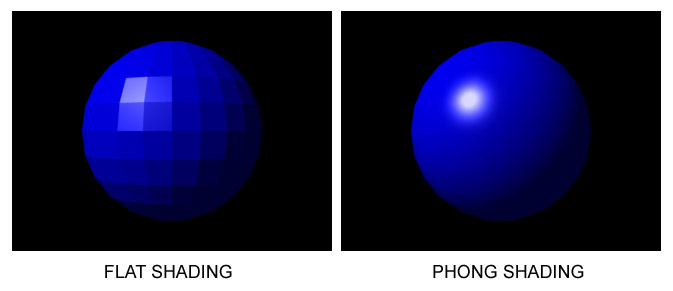
\includegraphics[width=\textwidth]{time_vs_quality}
    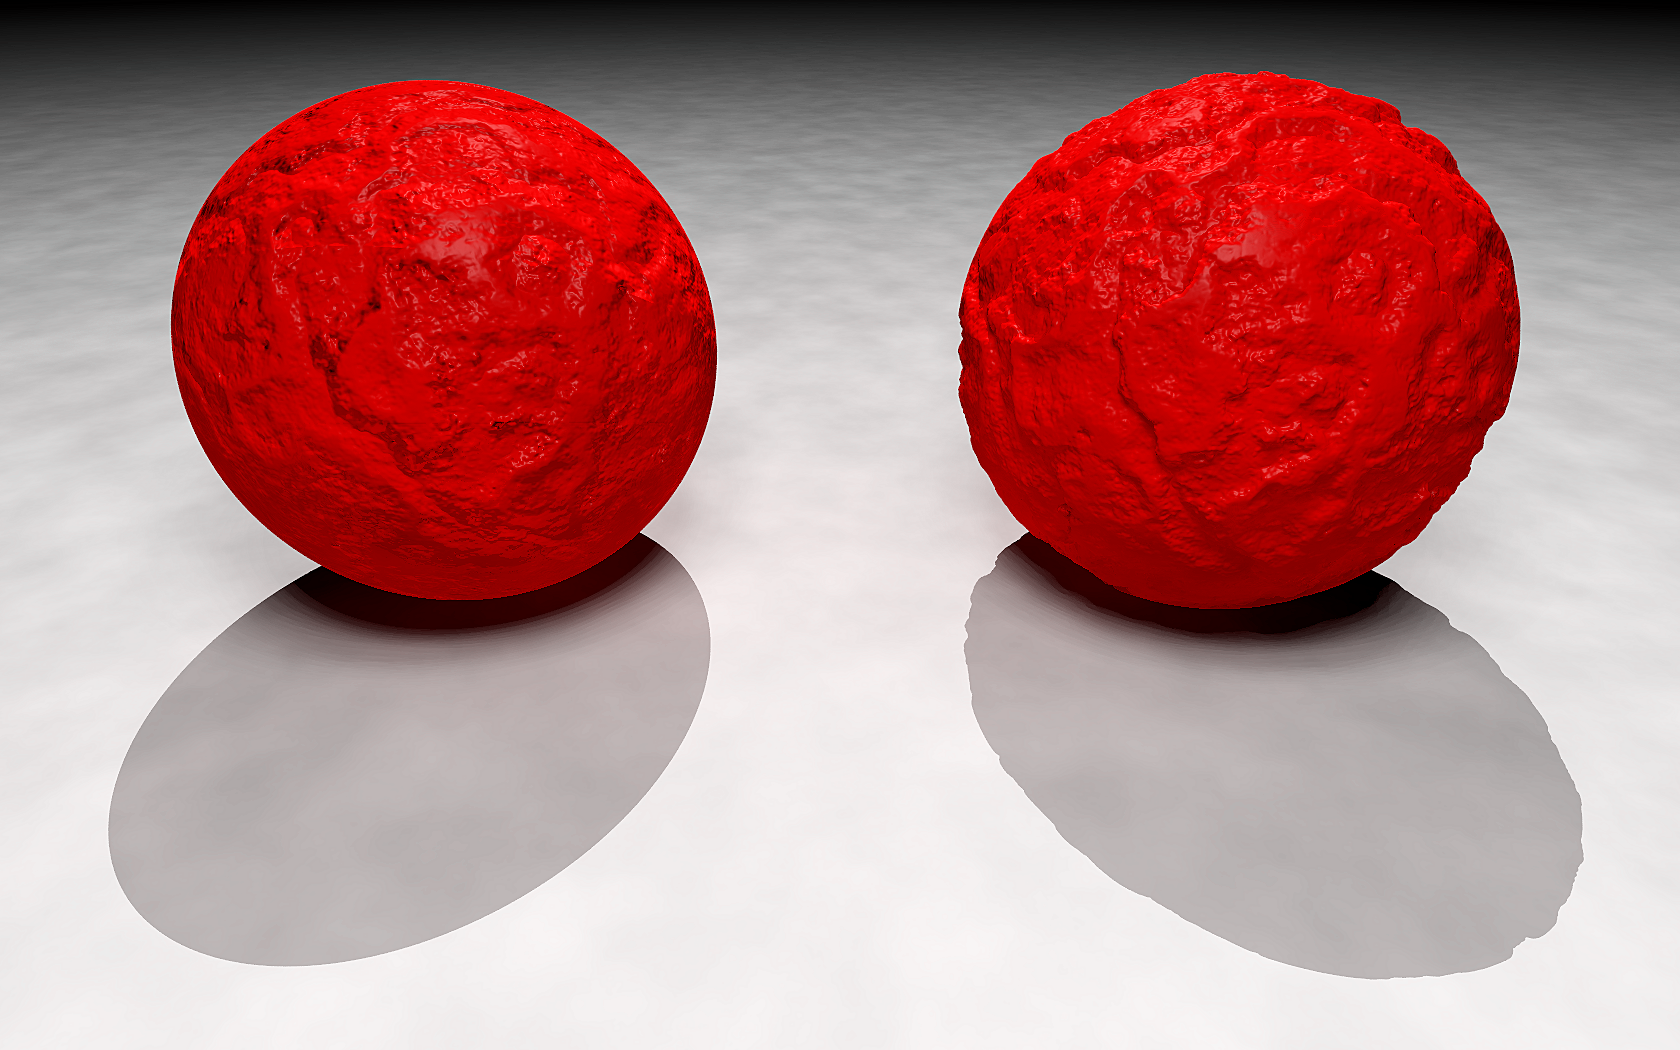
\includegraphics[width=\textwidth]{bumpmaps}
    \caption{Interpolation af flade-normaler kan få kantede figure til at få mere naturligt udseende.}
    \label{fig:tid_versus_kvalitet}
    % Demo der viser det samme http://math.hws.edu/graphicsbook/demos/c4/smooth-vs-flat.html
\end{figure}
\subparagraph{Rasterisering}
Den mest almindelige metode til at rendere miljøer med høj aktiv bruger interaktion er rasterisering. Rasterisering er også betegnelsen for at omdanne vector objekter til punkmatricer eller pixel-billeder (Se figur \ref{fig:pixelering}) Metoden virker ved at andvende linear transformationer på vektor objekter for at finde deres position på skærmen og derefter udfylde 2D polygonerne med farve, evt. baseret på forskællige lyskilder. Der kan dog simplificeres ved kun at andvende en ambient lys konstant. Rasterisering er også effektiv fordi grafikprocessore i computere er udviklet specifikt til at udføre matrix transformationer på store punktmængder.
\begin{figure}[H]
    \centering
    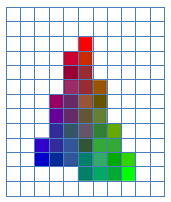
\includegraphics{rastarization_aprox}
    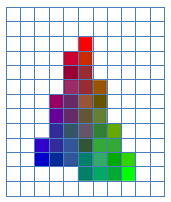
\includegraphics{rastarization_aprox}
    \caption{Pixelering der fremkommer når vektor objekter rastariseres.}
    \label{fig:pixelering}
\end{figure}
\subparagraph{Ray tracing}
% Kilder
% https://www.cs.unc.edu/~rademach/xroads-RT/RTarticle.html
% 
Raytracing er en metode som med relative simple regler, forsøger at andvende en fysisk model af lys, hvor fotoner spredes fra en lyskilde og rammer forskællige objekter indtil nogle få rammer øjet eller kamerarets optik. Raytracing simplificere ved at reducere problemet til kun at simulere de stråler der rammer vores øje. Dette gøres ved såkaldt \texit{backward ray tracing} hvorved man følger en stråle fra øjet, igennem computerskærmen og ind i vektormodellen hvor man tjekker for kollisioner mellem strålen og objekter. Ved kollision med reflektiktive objekter som metaliske overflader og gennemsigtige objekter som glas, vil strålen nu dele sig og følge f.eks gennem glasset men også følge en reflektiv vinkel for at udregne farven som den gennemsigtige/reflektive overflade har. For hver kollision følger man også en stråle mod alle lyskilder for at teste om der er objekter i vejen, således at kollisionspunktet ligger i skygge, da dette tages i betragtning som farven udregnes. Ved kollision med et mat objekt eller efter en forudbestemt antal reflektioner/refraktioner stopper udregningen og propagere tilbage igen.
\subparagraph{Radiosity}
% Kilder
% http://web.cs.wpi.edu/~matt/courses/cs563/talks/radiosity.html 
% http://www.cs.bath.ac.uk/~pjw/NOTES/75-ACG/ch5-radiosity.pdf
Hvor Rasterisering og raytracing udregner en pixels farve baseret på hvad man kan se igennem en skærmflade, så er radiosity en metode som er uafhængig af hvor kameraret er placeret og er af samme grund en af de mest tidskrævende metoder. (Måske er det muligt at precomputere modellen og så sende den til brugeren som kan interaktere med modellen via kameraret). Radiosity er baseret på en fysisk forståelse af lys interaktion med flader og fungere ved at alle flader absorbere en del af lyset der rammer dem og reflektere(radiates) resten som så går videre til at gentage processen for andre flader i scenen. Ved radiosity er lyskilder selv geometriske flader, hvilket gør det nemt at beskrive elementer som lamper og el-pærer. Karakteristisk for denne metode er såkaldt \textit{color bleeding}, hvor farver fra forskællige objekter smitter af på hindanden.
\begin{figure}[H]
    \centering
    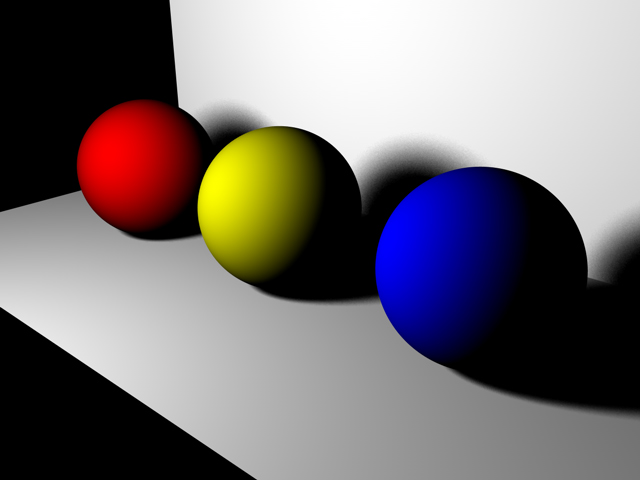
\includegraphics[width=6cm]{without_radiosity}
    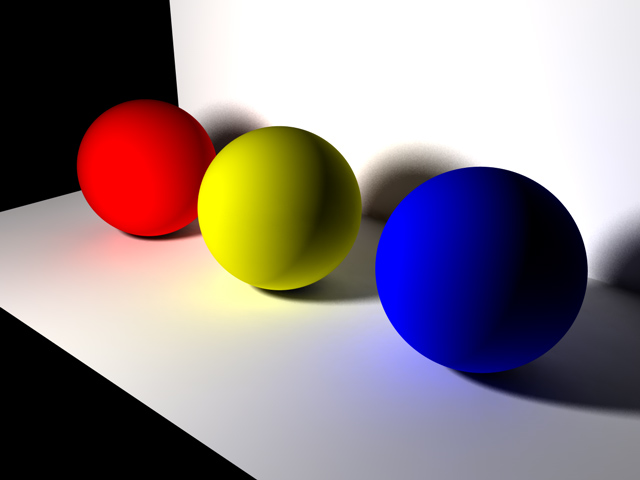
\includegraphics[width=6cm]{with_radiosity}
    \caption{\texit{Color bleeding} kan ses i billedet til højre.}
    \label{fig:colorbleeding}
\end{figure}

\clearpage


\section{Problemformulering}

Ud fra problemanalysen er vi blevet opmærksomme på følgende problem indenfor problemfeltet:
Det er et problem at kunden i en købssituation på e-butikker ikke kan visualisere, hvordan lys udbreder sig fra en lampe. Dette kan føre til fejlkøb af lamper, som påvirker både forbrugeren og e-butikken. For brugeren kan dette betyde irritation og i værste tilfælde kan det have sundhedsmæssige konsekvenser. For lampebutikker kan fejlkøb medføre utilfredse kunder og dårlig omtale. 

Dette fører os til det overordnede spørgsmål som vi ønsker besvaret i dette projekt:

\textit{Hvordan kan vi lave et værktøj til e-butikker, som vha.\ raytracing, visualiserer belysningen fra indendørslamper for kunderne?}

Herunder er der en række underspørgsmål, som ønskes besvaret:

\begin{enumerate}

\item \textit{Hvordan kan lampen visualiseres fra flere vinkler?}
\item \textit{Hvordan udbredes lyset fra en given lampe?}

\end{enumerate}

\section{Løsningsdesign}

\subsection{Teknologier til visualisering}
\label{sec:tek_til_visualisering}
Vi ser en tydelig mulighed for at assistere forbrugere med at træffe et valg, når det kommer til køb af varer på nettet. Formålet med afsnittet er, at få en forståelse af hvilke teknologier der allerede eksisterer inden for visualisering, og finde ud af hvilken teknologi, der er bedst i forhold til visualisering af lamper for kunder, der besøger en e-butiks hjemmeside. De enkelte teknologier vurderes på baggrund af de krav, der er sat til løsningsforslaget i afsnit \ref{sec:losning}.

\subsubsection{Digitale billeder taget med et fysisk kamera}
Som beskrevet under afsnit \ref{sec:ehandel}, benytter e-butikker, sig ofte af billeder til at vise kunden deres varer over internettet. Et eksempel på dette er vist på figur \ref{fig:e_handel_lampebilleder}.

\begin{figure}[H]
    \centering
    \fbox{\rule{\textwidth}{5cm}}
    \caption{Billeder af lamper på e-butikken somelampstore.what}
    \label{fig:e_handel_lampebilleder}
\end{figure} 

I det viste tilfælde er visualiseringen skabt ved at tage billeder af lamperne med et kamera fra en bestemt vinkel, i en kontekst, der typisk hænger sammen med lampetypen. 

Fordelen ved denne type af visualisering er, at den giver et virkelighedstro billede af, hvordan lampen ser ud i den kontekst, som billedet er taget i. Ulempen er, at der ofte kun er et begrænset antal billeder til rådighed, hvilket kan medføre, at forbrugeren ikke kan se lampen fra alle vinkler og på den måde ikke kan visualisere lampen for sig. Derudover kan det være svært, at se hvordan lyset udbreder sig fra lampen, da dette til dels afhænger af hvilken vinkel man ser lampen fra. 

Herudfra kan man kortfattet sige, at visualisering af lamper gennem billeder, taget med et fysisk kamera, giver et realistisk billede af lampen, men kun i den kontekst og vinkel billedet er taget i. 


\subsubsection{Computergrafik}
\label{sec:computergrafik}
I computergrafik, er en 3D model, en beskrivelse af objekters form og materiale \cite{computergrafik_introduktion}. Computergrafiske metoder kan bruges til at simulere, hvordan lys interagere med modellen og på den måde tegne et billede af modellen. Der eksisterer forskellige computergrafiske metoder, flere af hvilke kan bruges sammen med andre for, at opnå et mere realistisk eller effektivt resultat. Der er allerede værktøjer, som kan visualisere produkter til salg på websites som f.eks.\ Cylindo \cite{Cylindo}. Vi har ikke kendskab til at andre specialiserer sig, eller markedsfører sig på nuværende tidspunkt med deres kompetencer med fokus på visualisering af lampers belysning. Derfor er der herunder beskrivelse af to af de mest anvende metoder inden for computergrafik.

\paragraph{Rasterisering}
er en metode til at visualisere miljøer med høj aktiv brugerinteraktion som f.eks.\ computerspil \cite{rastarization}. Metoden virker ved rent matematisk at projektere modellen på et billedplan som repræsentere skærmen \cite{rastarization}. Fordelen ved rasterisering er at disse projektioner, kan foretages meget hurtigt af computerens grafikkort, som er bygget specielt til formålet \cite{rastarization}. Dette kan dog mindske fleksibiliteten, og muligheden for mere avancerede visualisering, hvor der kræves refleksioner og refraktioner af lys, som ikke passer ind i den proces (graphics pipeline \cite{rastarization}, som de enkelte grafikkort danner billeder ud fra). 

\paragraph{Ray tracing} [DER MANGLER KILDER TIL PÅSTANDE I DETTE AFSNIT]() forsøger, nøjagtigt at simulere lys i et virtuelt miljø, i modsætning til rasterisering hvor hastighed er den primære faktor. Raytracing bygger fundamentalt på at følge lysstråler og bygge en model for hvordan lysstrålerne interagere med forskellige objekter og materialer \cite{raytracing_for_begyndere}. 

I forhold til rasterisering, tager det længere tid at tegne, men komplekse lysfænomener som refleksioner og lys forvrængninger igennem semitransparante medier som vand(kaldet refraktion) er simple at beskrive for en raytracing algoritme, som kan tegne disse med realistisk precision. Nogle fænomener som bløde skygger kan også beskrives men jo flere typer fænomener og jo større realisme der kræves des længere tid tager det at tegne et billede, men raytracing tillader stor fleksibilitet.

\subsubsection{Augmented Reality}
Der er nu blevet gennemgået visualisering af virkelige objekter ved hjælp af digitale billeder og virtuelle objekter ved hjælp af computergrafik. I dette afsnit beskrives augmented reality som er en teknologi der kombinerer virkelige og virtuelle objekter \cite{augmented_reality}.

Augmented reality fungerer ved at tage et billede med et normalt kamera, og herefter ændrer billedet ved at indsætte computergrafik på billedet \cite{augmented_reality}.

Et eksempel på anvendelsen af augmented reality er Artemides Augmented Reality App. Denne app gør det muligt, at visualisere udvalgte lamper i en kontekst som brugeren selv vælger \cite{artemides}. 

Fordelen ved augmented reality i forhold til løsningsforslaget er, at den muliggøre at se lampen fra flere forskellige vinkler i den kontekst som kunden ønsker. Hvis der ses bort fra tekniske udfordringer så ville det også være en fordel hvis kunden kunne visualisere en lampe og dens belysning i den kontekst som kunden ønsker at købe lampen til. \newline Ulempen ved augmented reality i forhold til løsningsforslaget er, at det er en teknisk udfordring, at få en rummelig forståelse for den virkelig kontekst så det virtuelle der indsættes får en tilstrækkelig realisme. Det vil derfor være svært at simulere lampens belysning hvis man ikke kender til dimensioner eller materialerne i den virkelige kontekst. Hvis det lykkedes, at få en forståelse for de virkelige objekter i billedet, så vil det stadigvæk være raytracing eller en anden teknik indenfor computergrafik som ville være at foretrække når man skal visualisere lampens belysning. Derfor er udfordringen ved augmented reality dobbelt, da den både skal få en rummelig forståelse for de virkelige objekter i billedet, samt lave en realistisk computergrafik som passer ind i billedet.



\subsubsection*{Opsummering}
Ud fra ovenstående afsnit er der udledt følgende fordele og ulemper for de enkelte teknologier.
\begin{table}[H]
  \centering
  
\center
    \begin{tabular}{ | p{3cm} | p{5cm} | p{5cm} |}
    
    \hline
    Teknologi & Fordele & Ulemper \\ \hline
    Kamerabilleder & Realistisk visualisering. & Tidskrævende. Begrænset kombinationer af lampen, synsvinkel, farvetemperatur og kontekst. \\ \hline
   Computergrafik & Nemt at integrere på lampebtuikker hjemmesider. Kan opnå høj realisme af lampen og dens belysning. \newline Nemt at ændre vinkel, farvetemperatur og kontekst hvorfra lampen visualiseres. & Kræver 3D-model af lampen og konteksten. Kræver meget computerkraft ved høj realisme. \\ \hline
   Augmented Reality & Lampen kan visualiseres fra flere vinkler og i den kontekst som kunden ønsker at købe lampen til. & Det er en teknisk udfordring at virtuelle objekter med den virkelige kontekst, så der stadigvæk opnås en hvis realisme. \\ \hline
    \end{tabular}
  \caption{Viser fordele og ulemper ved de tre teknologier til visualisering.}
\label{tab:fordele_ulemper_teknologier}
\end{table}

På baggrund af fordele og ulemper vist i tabel \ref{tab:fordele_ulemper_teknologier} sammenlignes de tre teknologier nu med de krav, der er opstillet til løsningsforslaget i afsnit \ref{sec:losning}. 

Billeder af fysiske lamper taget med et kamera, kan bidrage til udviklingen af løsningsforslaget, da den delvist opfylder krav 1-3 og 5. Da det er muligt at tage et billede af lampen og dens belysning med en bestemt farvetemperatur og fra en bestemt vinkel. Derudover kan løsningen implementeres på en e-butikshjemmeside, ved blot at bruge de billeder, der tages med kameraet. Ulempen er, at det kan være ressourcekrævende, da der skal tages billeder med forskellige lamper, farvetemperaturer og vinkler som giver mange kombinationer og dermed mange billeder.

Hvordan computergrafik kan biddrage med at løse kravene i afsnit \ref{sec:losning}, afhænger af hvilken teknik man benytter. Hvis man benytter rasterisering, vil det være svært at opfylde krav 1, da visualisering af lampens belysning kræver, at der anvendes lysfænomener, som ikke passer ind i modellen for rasterisering. Rasterisering vil dog være oplagt til at opfylde krav 2 og 4, da den som nævnt er bygget til at rendere et billede med høj brugerinteraktion og kort renderingstid.
Raytracing vil derimod være oplagt til at opfylde krav 1-3, da det er muligt at simulere lampen og dens belysning med forskellige farvetemperaturer og vinkler. Derudover kan raytracing implementeres i løsningen, der renderer et billede, der kan vises på en e-butikshjemmeside, hvilket gør at den opfylder krav 5. Ulempen ved raytracing er, at det kan være svært at opfylde krav 4, da simulering af lampens belysning kan være en tidskrævende proces.

Augmented reality kan bidrage til udviklingen af løsningsforslaget ved at den har potentialet for at opfylde de samme krav, som både visualisering vha.\ kamerabilleder og computergrafik (krav 1-3). Dog er dette en teknisk udfordring, da den rummelige forståelse af den virkelige kontekst af billedet er nødvendig for at kunne opnå en realistisk visualisering, når computergrafikken indsættes. I forhold til krav 4 har augmented reality den samme udfordring som f.eks.\ raytracing, da simulering af lampens belysning kan være en tidskrævende proces. Derudover kan det være svært at implementere augmented reality på en e-butikshjemmeside, da det kræver adgang til kundens kamera. Ud fra ovenstående har vi valgt raytracing som teknologi til visualisering, da den har potentialet for at opfylde kravene opstillet i afsnit \ref{sec:losning}, uden at være en lige så stor teknisk udfordring som augmented reality. 


\clearpage



\subsection{Ide}

I dette afsnit er der beskrevet en ide til løsningen af den endelige problemformulering. Ideen er resultatet af en diskussion i gruppen, hvor vi kom med ideer til løsninger, og herefter diskuterede fordele og ulemper ved de forskellige ideer. Formålet med afsnittet er at skitsere gruppens bud på den optimale løsning på problemet, og afsnittet er derfor udarbejdet med feedback fra forskellige lampebutikker. I slutningen af afsnittet vil der være en afgrænsning af løsningen som vil danne grundlag for den senere udvikling af en løsning.

Den løsning som gruppen har valgt at arbejde med er, "3D modeller af lamper med interaktion". Som beskrevet i problemanalysen har gruppen valgt at løse problemet når kunder handler på e-butikker. Tanken er derfor at implementere software på en e-butiks hjemmeside med henblik på at løse problemet for kunden.

\subsubsection{Skitse af løsning}

\begin{figure}[H]
   \centering
   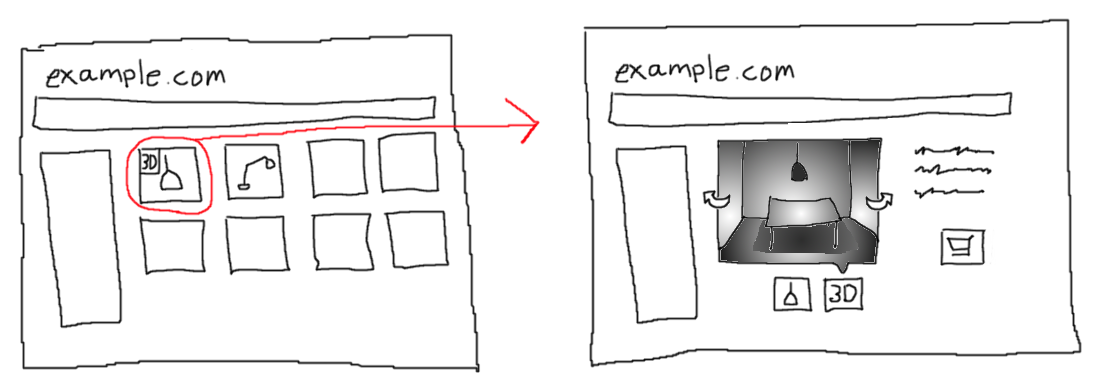
\includegraphics[width=\textwidth]{skitse_til_loesning}
   \caption{Skitse af ide til løsning.}
\end{figure}

På figur 5 er der illusteret en skitse af en e-butik som sælger lamper. Figuren illustrerer hvordan systemet kan integreres på en hjemmeside. Skitse 5a viser et online katalog over e-butikkens udvalg af lamper. Som der fremgår af skitsen vil nogle lamper være markeret med et "3D-ikon" og dette indikerer, at kunden har mulighed for, at se skitsen i 3D. Kunden tilgår 3D-billedet ved at klikke på ikonet. Når kunden trykker på ikonet bliver kunden omdirigeret til en anden menu. Som der fremgår af skitse 5b, så har kunden her mulighed for at se en 3D-model af lampen i et rum. De to pile på skitsen indikerer, at kunden har mulighed for at rotere billedet, og se hvordan belysningen fra lampen er, set fra forskellige vinkler. Som en ekstra feature har kunden mulighed for at indtaste en kontekst, beskrevet som en model, ind i programmet og har derefter mulighed for at se hvordan lampen ser ud i den kontekst som kunden ønsker. 
Derudover har kunden mulighed for, at justere lampens farvetemperatur (i kelvin), meningen med denne feature er, at kunden har mulighed for at visualisere hvordan forskellige pærer vil se ud i lampen. De forskellige 3D billeder vil ligge til rådighed på en ekstern server og vil derfor ikke gøre e-butikkernes hjemmeside betydeligt langsommere. Derudover er tanken af alle 3D billeder bliver udleveret af producenten af lamperne. 

\begin{figure}[H]
   \centering
   
\includegraphics[width=\textwidth]{brugerinteraktion}
   \caption{Sekvensdiagram af løsningsideen.}
\end{figure}

Figur 6 tager udgangspunkt i en hjemmeside som har fået implementeret vores løsning, og viser et sekvensdiagram som illustrere processen når en kunde vil købe en lampe.  

I forbindelse med implementeringen af softwaren på en hjemmeside har der været forskellige ting som skulle overvejes. Da problemet omhandler visualisering af lys fra lamper, har gruppen valgt at fokusere på at lave en løsning hvis primære formål er at generere realistiske 3D-billeder af lamper. Disse billeder vil vise belysningen fra lamper med forskellige pærer. Features som interaktion og kontekst, har derfor anden priotet. 

Ud fra ovenstående beskrivelse har gruppen derfor valgt, i første omgang, at fokusere på at lave et program der gør det muligt for kunden, at visualisere hvordan lys spreder sig fra lamper illustreret igennem realistiske 3D-billeder. Derudover har kunden mulighed for at justere pærens farvetemperatur, og derved også se hvordan lampens belysning med forskellige pærer.  


\subsubsection{Krav til løsningen}

I forbindelse af vores projekt har vi fået nogle krav fra universitetets side. Disse er at programmet skal skrives i programmeringssproget C, derudover er der også tidsmæssigt pres da hele projektet kun varer ca.\ to en halv måned. 
Vi er også begrænset af vores egen viden indenfor emnet, da raytracing er en fremmed teknik, som få af os har haft tidligere erfaringer med. 

Vi har selv opstillet nogle krav til vores program for hvad vi mener programmet skal kunne før det kan være et færdigt produkt.
\begin{enumerate}
    \item Programmet skal kunne implementeres på en hjemmesiden (ellers bruges på en computer i den fysiske butik).
    \item skal kunne visualisere billedet relativt hurtigt, da kunderne ikke skal vente før de kan se billedet.
    \item Programmet skal kunne modtage et vilkårligt billede (i den rigtige format) og renderer dette.
    \item Lysets udbreddelse skal kunne ses tydeligt af kunden.
    \item Det skal være muligt for kunden skal kunne ændre farvetemperatur.
    \item Det skal være muligt for kunden at rotere billedet.
    \item Det skal være muligt for kunden at kunne indsætte en vilkårlig kontekst.
    \item Programmet skal være let at bruge, så en potentiel kunde ikke vil blive frusteret og derved vil forlade butikken/siden.
    \item 
\end{enumerate}

\subsubsection*{Opsummering}
[Kort opsummering af præcist ideen bag løsningen]

\clearpage

\section{Problemløsning}

[Indledning til overafsnittet problemløsning]

\subsection{Teknologier til visualisering}
\label{sec:teknologianalyse}
Vi ser en tydelig mulighed for at assistere forbrugere med at træffe et valg, når det kommer til køb af varer på nettet. For at undersøge hvilke teknologier, der kan anvendes til visualisering, er der i dette afsnit en række teknologier og metoder, som alle er relevante i forhold til at visualisere en lampe. Teknologierne er udvalgt på baggrund af diskussion i gruppen, hvor mindre relevante teknologier, som f.eks. 3D-print blev fravalgt. Formålet med afsnittet er, at få en forståelse af hvilke teknologier der allerede eksisterer inden for visualisering, og finde ud af hvilke metoder, der er bedst i forhold til visualisering af lamper for brugere der handler via internettet.

\subsubsection{Digitale billeder taget med et fysisk kamera}
Som beskrevet under afsnit \ref{sec:ehandel}, benytter e-butikker, sig ofte af billeder til at vise kunden deres varer over internettet. Et eksempel på dette er vist på figur \ref{fig:e_handel_lampebilleder}.

\begin{figure}[H]
    \centering
    \fbox{\rule{\textwidth}{5cm}}
    \caption{Billeder af lamper på e-butikken somelampstore.what}
    \label{fig:e_handel_lampebilleder}
\end{figure} 

I det viste tilfælde er visualiseringen skabt ved at tage billeder af lamperne med et kamera fra en bestemt vinkel, i en kontekst, der typisk hænger sammen med lampetypen. 

Fordelen ved denne type af visualisering er, at den giver et virkelighedstro billede af, hvordan lampen ser ud i den kontekst, som billedet er taget i. \newline Ulempen er, at der ofte kun er et begrænset antal billeder til rådighed, hvilket kan medføre, at forbrugeren ikke kan se lampen fra alle vinkler og på den måde ikke kan visualisere lampen for sig. Derudover kan det være svært, at se hvordan lyset udbreder sig fra lampen, da dette til dels afhænger af hvilken vinkel man ser lampen fra. 

Herudfra kan man kortfattet sige, at visualisering af lamper gennem billeder, taget med et fysisk kamera, giver et realistisk billede af lampen, men kun i den kontekst og vinkel billedet er taget i. 

% \subsubsection{3D print}
% En teknologi, som lampebutikker vil kunne bruge, er 3D printere. 3D printere anvender plastik istedet for blæk, som bliver varmet op til knap 200 grader \cite{hvordan_3Dprinter}. Den flydende plastik bliver lagt i tynde lag og størkner hurtigt efter at have bundet sig med det underliggende lag. 

% Sælgeren kan give forbrugeren en fil, så forbrugeren selv vil være i stand til at lave et 3D print af en bestemt lampe. Dette forudsætter dog, at forbrugeren har en 3D printer og, at brugeren er dedikeret nok til at få printet lampen, da store objekter kan tage dage at printe og ofte skal deles op i mindre dele.\cite{hvordan_3Dprinter}. Derudover er 3D printere stadig en så ny teknologi, og de er stadig primært rettet mod hobbyfolk som vil bruge lang tid på, at få kallibreret printeren korrekt, da et print ellers nemt kan fejle. 3D printer er heller ikke en billig inverstering, da nogle modeller koster over titusinde kroner\cite{3D_printer}. 

% Idag vil det være en dårlig ide for lampebutikker at forvente, at deres kunder har en 3D printer derhjemme. Et andet problem er, at lampebutikker også kommer i et dilemma, da lampebutikker skal bestemme om man kan udgive tegninger inden forbrugeren har købt lampen eller om de skal betale en form for depositum.

\subsubsection{Computergrafik}
\label{sec:computergrafik}
I computergrafik, er en 3D model, en beskrivelse af objekters form og materiale.\cite{computergrafik_introduktion} Computergrafiske metoder kan bruges til at immitere hvordan lys interaktere med modellen og på den måde tegne et billede af modellen. Der eksisterer en mængde forskellige computergrafiske metoder, flere af hvilke kan bruges sammen med andre for, at opnå et mere realistisk eller effektivt resultat. Der findes flere produkter som kan visualisere produkter til salg på websites som f.eks. Cylindo\cite{Cylindo}. Men vi har ikke kendskab til at andre specialisere sig, eller markedsføre sig på nuværende tidspunkt med deres kompetencer med fokus på visualisering af lampers belysning.

\paragraph{Rasterisering}
er en metode til at visualisere miljøer med høj aktiv brugerinteraktion som f.eks. computerspil.\cite{rastarization} Metoden virker ved rent mattematisk at projektere modellen på et billedplan som repræsentere skærmen.\cite{rastarization}. Fordelen ved rasterisering er at disse projektioner, kan foretages meget hurtigt af computerens grafikkort, som bygget specielt til formålet\cite{rastarization}.\newline Ulempen er, at dette kan mindske fleksibiliteten, og muligheden for mere avancerede visualisering, hvor der kræves refleksioner og refraktioner af lys, som ikke passer ind i den proces (graphics pipeline\cite{rastarization}, som de enkelte grafikkort danner billeder ud fra. 

\paragraph{Ray tracing}\cite{raytracing_for_begyndere} forsøger, nøjagtigt at simulere lys i et virtuelt miljø, i modsætning til rasterisering hvor hastighed er den primære faktor. Raytracing bygger fundementalt på at følge stråler af lys og bygge en model for hvordan de stråler interagere med forskellige objekter og materialer. Der skælnes mellem to typer af raytracing: Forwards raytracing og backwards raytracing.

\subparagraph{Forwards raytracing}\cite{radiosity_by_wpi,radiosity_by_uob} er oftere kaldet radiosity og vil bliver reffereret til som sådan fremhenværende. Radiosity er hvad man kunne kalde en forwards raytracing metode. Her eksistere lyskilder ikke som specielle objekter i en 3D model, hvilket er tilfældet for de andre metoder, men her som objekter uden forskel fra de andre i modellen.

I radiosity modellen er alle flader betegnet med en absorbans faktor og en energi faktor. Absorbansen beskriver hvor meget af lys der rammer fladen der bliver absorberet. Absorberet lys hæver en flades energi og som i virkeligheden, afgives noget af den energi som lys, mens andet bliver omdannet til f.eks. varme. Lyskilder er således blot flader som starter med en mængde energi.

Radiosity er i stor grad blandt de mest tidskrævende metoder eftersom at den laver beregninger som ikke nødvendigvis bliver set i et billede. Dette muliggøre dog at visualisere en scene en gang og derefter at kunne se den fra mange vinkler eftersom at de ekstra udregninger allerede er gjort. Radiosity er derimod ikke designet til at håndtere fænomener som er afhængig af hvor man ser et objekt fra, så som refleksion og refraktion. Dvs. at radiosity ikke kan håndtere metalliske overflader eller semitransparente materialer. Til gengæld er Radiosity rigtig god til at simulere matte overflader og skygger.

\subparagraph{Backwards raytracing} er hvad man i almindelighed kalder raytracing og vil bliver reffereret til som sådan fremhenværende. Raytracing forsøger at simplificerer den fysiske model af lys ved at ignorere det lys som ikke rammer vores øjne. Raytracing er dog alligevel blandt de metoder som kendes for at kunne skabe de mest fotorealistiske renderinger. Dette gøres ved såkaldt \textit{backwards raytracing}, hvorved man følger en stråle fra øjet og ud mod 3D modellen, så tjekkes der for kollisioner mellem strålen og objekterne i modellen. Ved hver kollision kan man vælge at følge yderligere stråler som kan hjælpe med at udregne refleksioner eller komplekse skygger. Denne metoder står i modsætning til hvad man kalder \textit{forwards raytracing} som er den mere fysisk korrekte metode, hvor man følger stråler af lys fra hver lyskilde.

I forhold til rasterisering, tager raytracede billeder væsentligt længere tid at tegne, men komplekse lysfænomener som refleksioner og lys forvrængninger igennem semitransparante medier som vand(kaldet refraktion) er simple at beskrive for en raytracing algoritme, som kan tegne disse med realistisk precision. Nogle fænomener som bløde skygger kan også beskrives men jo flere typer fænomener og jo større realisme der kræves des længere tid tager det at tegne et billede, men raytracing tillader stor fleksibilitet.

\subsubsection{Augmented Reality App}

Augmented Reality er en teknologi der kan sætte virtuelle objekter ind i en virkelig kontekst. Derudover har man mulighed for at interagere med objektet i real tid. 
Denne metode bruger producenten "Artemides" i deres Augmented Reality App. Appen virker ved, at man scanner et logo fra et fysisk lampekatalog, hvorefter en givet lampe vil vise sig på logoets plads. Det er herefter muligt at flytte kataloget for, at se lampen i forskellige kontekster. Derudover har man mulighed for at rotere i alle vinkler samt tænde og slukke for lampens pære. 
Fordelene ved appen er, at brugeren har mulighed for selv at vælge hvilken lampe de vil se i sin egen kontekst, samt interagere med lampen. Herved har brugeren mulighed for, at se præcist hvordan lampen ser ud. 
Ulemperne ved appen er, at den ikke visualisere lampens belysning særlig godt, da dens første priotet er at visualisere selve lampens design. Derudover er det ikke muligt at visualisere lamper i en kontekst, hvis man ikke har den nødvendige bog som indeholder logoer over de forskellige lampedesigns i 3D. En anden ulempe er, at lampeudvalget er meget begrænset da det kun er udvalgte produkter fra "Artemides" som kan visualiseres. 
Nedenstående figur viser "Artemides" brugervejledning til appen.

\begin{figure}[H]
    \centering
    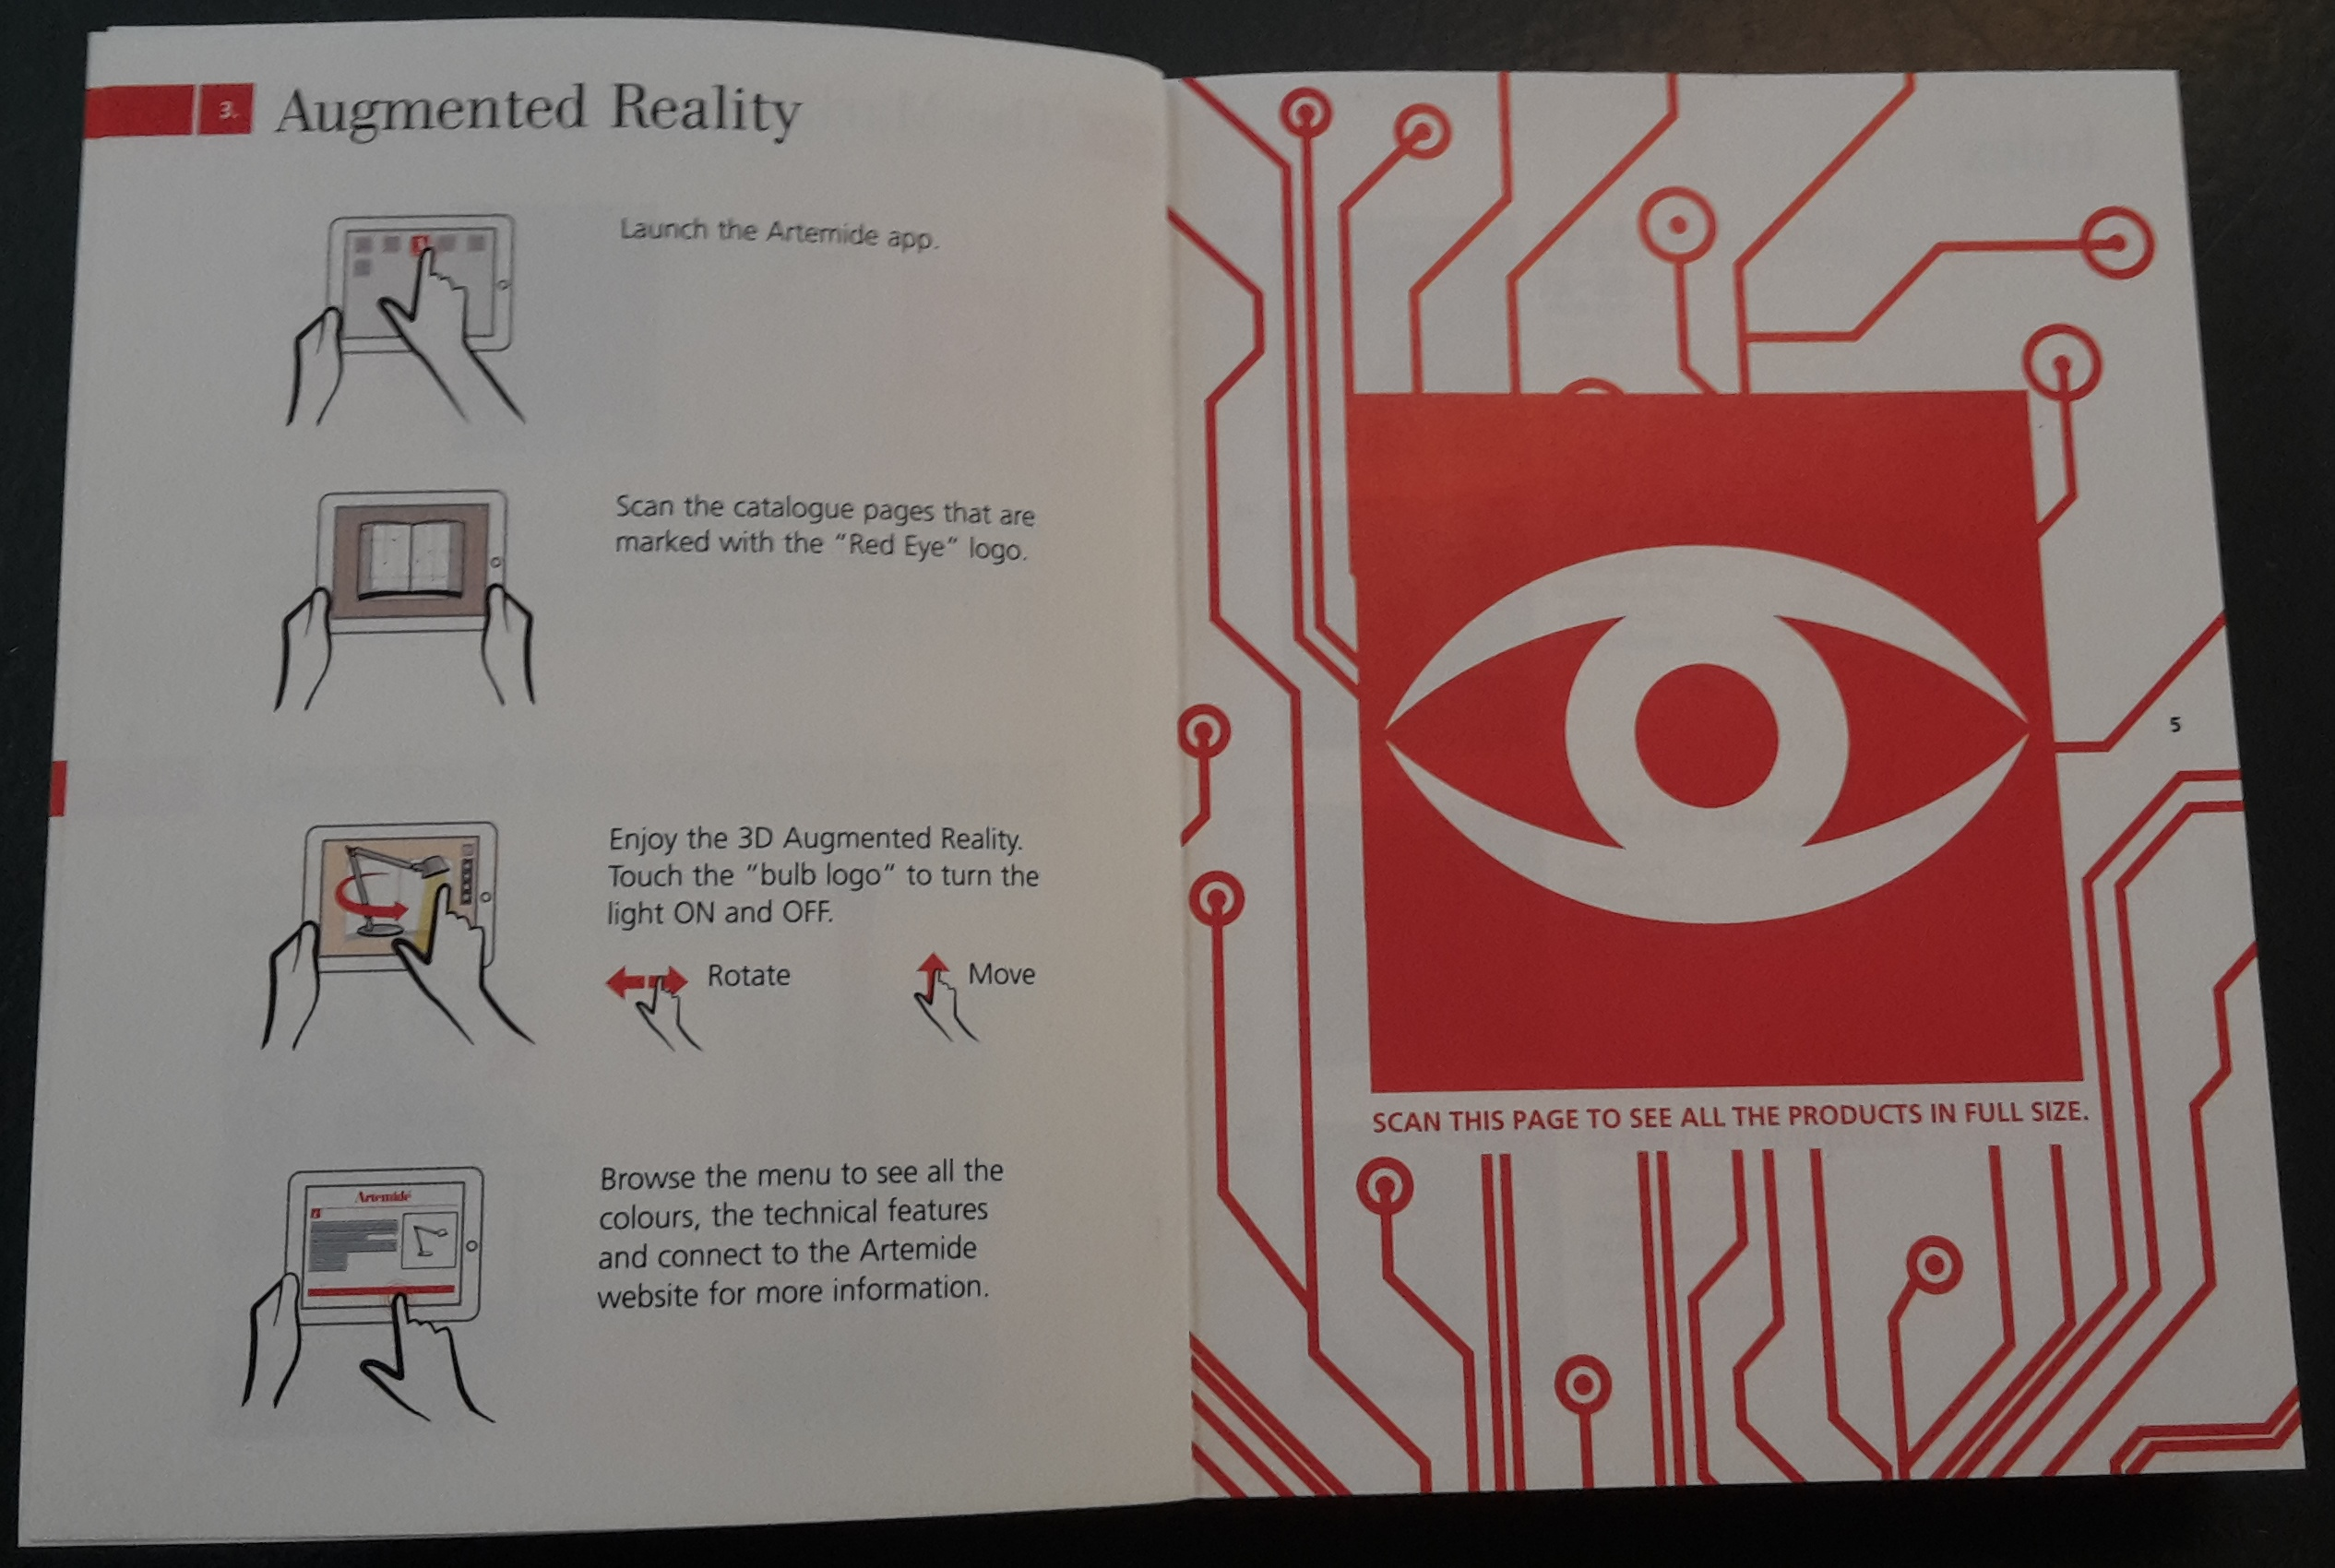
\includegraphics[width=10cm]{augmented_reality_artemides}
    \caption{Brugervejledning fra Artemides augmented reality.}
    \label{fig:augmented_reality_artemides}
\end{figure} 


\subsubsection*{Opsummering}
Billeder af den fysiske lampe er gode til akkurat at gengive lampen, men det er et problem at der ofte ikke er billeder nok fra forskellige vinkler, at billederne kun viser lampens form og ikke dens lys og at det er for besværligt at tage billeder af lampen med forskellige pærer for at vise forskellige farvetemperature og at det også er bbesværligt at udskifte den kontekst som lampen bliver vist i. 

Computergrafik kan nemt indlejres i en hjemmeside. Hvilken Computergrafisk teknik der er den korrekte er et case til case valg eftersom det helt afhænger af hvor meget fleksibilitet versus kvalitet der er nødvendigt. Rasterisering og radiosity kan begge implementeres på en måde hvorved der opnås et højt niveau af bruger interaktion som kan gøre værktøjet mere naturligt at anvende for forbrugeren. Eftersom at målet er at simulere lamper og ikke møbler som borde og stole, er langt mere komplekst at lave en god visualisation med rasterisering. Radiosity falder også til kort hvis der er behov for mere komplekse materialer som metalliske overflader eller f.eks. klar plast og glas. Billeder tegnet med raytracing kan tage lang tid at rendere, men der er mulighed for stor fleksibilitet og komplekse materialer er relativt simple at rendere. Med det grundlag vil rapporten fremadrettet arbejde med raytracing som metode til visualisering.

\subsection{Ide}

\subsection{Ide}

I dette afsnit er der beskrevet en ide til løsningen af den endelige problemformulering. Ideen er resultatet af en diskussion i gruppen, hvor vi kom med ideer til løsninger, og herefter diskuterede fordele og ulemper ved de forskellige ideer. Formålet med afsnittet er at skitsere gruppens bud på den optimale løsning på problemet, og afsnittet er derfor udarbejdet med feedback fra forskellige lampebutikker. I slutningen af afsnittet vil der være en afgrænsning af løsningen som vil danne grundlag for den senere udvikling af en løsning.

Den løsning som gruppen har valgt at arbejde med er, "3D modeller af lamper med interaktion". Som beskrevet i problemanalysen har gruppen valgt at løse problemet når kunder handler på e-butikker. Tanken er derfor at implementere software på en e-butiks hjemmeside med henblik på at løse problemet for kunden.

\subsubsection{Skitse af løsning}

\begin{figure}[H]
   \centering
   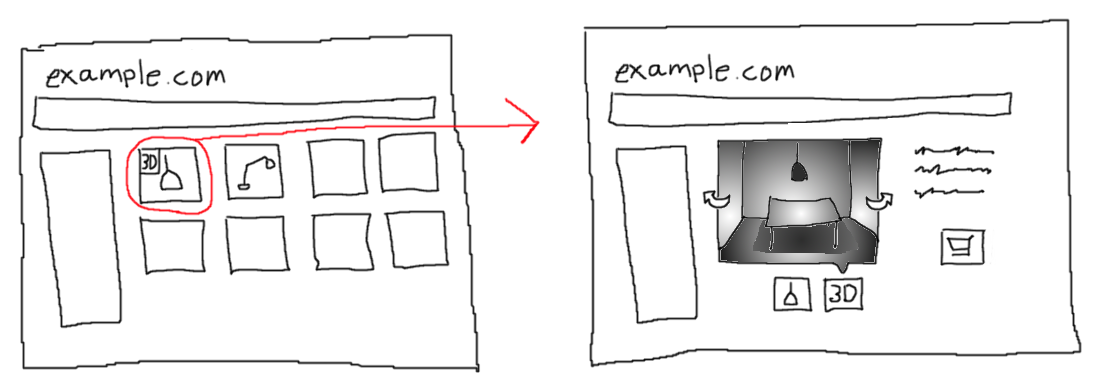
\includegraphics[width=\textwidth]{skitse_til_loesning}
   \caption{Skitse af ide til løsning.}
\end{figure}

På figur 5 er der illusteret en skitse af en e-butik som sælger lamper. Figuren illustrerer hvordan systemet kan integreres på en hjemmeside. Skitse 5a viser et online katalog over e-butikkens udvalg af lamper. Som der fremgår af skitsen vil nogle lamper være markeret med et "3D-ikon" og dette indikerer, at kunden har mulighed for, at se skitsen i 3D. Kunden tilgår 3D-billedet ved at klikke på ikonet. Når kunden trykker på ikonet bliver kunden omdirigeret til en anden menu. Som der fremgår af skitse 5b, så har kunden her mulighed for at se en 3D-model af lampen i et rum. De to pile på skitsen indikerer, at kunden har mulighed for at rotere billedet, og se hvordan belysningen fra lampen er, set fra forskellige vinkler. Som en ekstra feature har kunden mulighed for at indtaste en kontekst, beskrevet som en model, ind i programmet og har derefter mulighed for at se hvordan lampen ser ud i den kontekst som kunden ønsker. 
Derudover har kunden mulighed for, at justere lampens farvetemperatur (i kelvin), meningen med denne feature er, at kunden har mulighed for at visualisere hvordan forskellige pærer vil se ud i lampen. De forskellige 3D billeder vil ligge til rådighed på en ekstern server og vil derfor ikke gøre e-butikkernes hjemmeside betydeligt langsommere. Derudover er tanken af alle 3D billeder bliver udleveret af producenten af lamperne. 

\begin{figure}[H]
   \centering
   
\includegraphics[width=\textwidth]{brugerinteraktion}
   \caption{Sekvensdiagram af løsningsideen.}
\end{figure}

Figur 6 tager udgangspunkt i en hjemmeside som har fået implementeret vores løsning, og viser et sekvensdiagram som illustrere processen når en kunde vil købe en lampe.  

I forbindelse med implementeringen af softwaren på en hjemmeside har der været forskellige ting som skulle overvejes. Da problemet omhandler visualisering af lys fra lamper, har gruppen valgt at fokusere på at lave en løsning hvis primære formål er at generere realistiske 3D-billeder af lamper. Disse billeder vil vise belysningen fra lamper med forskellige pærer. Features som interaktion og kontekst, har derfor anden priotet. 

Ud fra ovenstående beskrivelse har gruppen derfor valgt, i første omgang, at fokusere på at lave et program der gør det muligt for kunden, at visualisere hvordan lys spreder sig fra lamper illustreret igennem realistiske 3D-billeder. Derudover har kunden mulighed for at justere pærens farvetemperatur, og derved også se hvordan lampens belysning med forskellige pærer.  


\subsubsection{Krav til løsningen}

I forbindelse af vores projekt har vi fået nogle krav fra universitetets side. Disse er at programmet skal skrives i programmeringssproget C, derudover er der også tidsmæssigt pres da hele projektet kun varer ca.\ to en halv måned. 
Vi er også begrænset af vores egen viden indenfor emnet, da raytracing er en fremmed teknik, som få af os har haft tidligere erfaringer med. 

Vi har selv opstillet nogle krav til vores program for hvad vi mener programmet skal kunne før det kan være et færdigt produkt.
\begin{enumerate}
    \item Programmet skal kunne implementeres på en hjemmesiden (ellers bruges på en computer i den fysiske butik).
    \item skal kunne visualisere billedet relativt hurtigt, da kunderne ikke skal vente før de kan se billedet.
    \item Programmet skal kunne modtage et vilkårligt billede (i den rigtige format) og renderer dette.
    \item Lysets udbreddelse skal kunne ses tydeligt af kunden.
    \item Det skal være muligt for kunden skal kunne ændre farvetemperatur.
    \item Det skal være muligt for kunden at rotere billedet.
    \item Det skal være muligt for kunden at kunne indsætte en vilkårlig kontekst.
    \item Programmet skal være let at bruge, så en potentiel kunde ikke vil blive frusteret og derved vil forlade butikken/siden.
    \item 
\end{enumerate}

\subsubsection*{Opsummering}
[Kort opsummering af præcist ideen bag løsningen]

\subsubsection{Krav til løsningen}

%\subsection{krav}

I forbindelse af vores projekt har vi fået nogle krav fra universitetets side. Disse er at programmet skal skrives i programmeringssproget C, derudover er der også tidsmæssigt pres da hele projektet kun varer ca to en halv måned. 
Vi er også begrænset af vores egen viden indenfor emnet, da raytracing er en fremmed teknik, som få af os har haft tidligere erfaringer med. 



\subsubsection*{Opsummering}

[Kort opsummering af præcist ideen bag løsningen]

\subsection{Teori}

\subsubsection{Rotationsmatricer}

\subsubsection{Rotationsmatricer}
\label{sec:rot_matricer}
Hvis vi vil rotere et punkt eller en vektor omkring nul-punktet i et koordinatsystem kan vi bruge en rotationsmatrix \cite{rotationsmatricer}.
En rotationsmatrix er en matrix, der, hvis multipliceret sammen med en anden matrix, roterer en vektor eller et punkt i et koordinatsystem.
\begin{align} \label{eu_eqn}
  R_x(\theta) = 
  \begin{bmatrix}
  \label{eq:rotate_around_x}
    1 & 0 & 0\\ 
    0 & cos \theta & - sin \theta\\ 
    0 & sin \theta & cos \theta
  \end{bmatrix}\\
    R_y(\theta) =
  \begin{bmatrix}
    cos \theta  & 0 & sin \theta\\ 
    0           & 1 & 0\\ 
    -sin \theta & 0 & cos \theta
  \end{bmatrix}\\
    R_z(\theta) = 
  \begin{bmatrix}
    cos \theta & - sin \theta & 0\\ 
    sin \theta & cos \theta & 0\\
    0 & 0 & 1
  \end{bmatrix}
\end{align}
Vi indsætter den vinkel som vi vil dreje vektoren med i radianer og multiplicerer dem sammen som angivet i udtryk \ref{eq:rotate_around_x}. Vektoren bliver drejet omkring nul-punktet med netop den mængde radianer, som er angivet.
Nedenstående eksempel illustrerer princippet ved at dreje en vektor i rummet.

\begin{equation}
  {\vv{u}} =
  \begin{bmatrix}
    u_x \\ 
    u_y \\
    u_z
  \end{bmatrix}
\end{equation}
og rotationsvektor \begin{math}R_x\end{math}
\begin{equation}
  R_x(\theta) = 
  \begin{bmatrix}
    1 & 0 & 0\\ 
    0 & cos \theta & - sin \theta\\ 
    0 & sin \theta & cos \theta
  \end{bmatrix}
\end{equation}
Den roterede vektor $\vv{u}$ kan nu beskrives som set i udtryk \ref{eq:rotation_x}
\begin{equation}
  \vv{v} = R_x(\theta) \cdot \vv{u} = \begin{bmatrix}
    u_x \\ 
    cos(\theta)   \cdot u_y - sin(\theta) \cdot u_z \\
    sin(\theta) \cdot u_y + cos(\theta) \cdot u_z
  \end{bmatrix}
  \label{eq:rotation_x}
\end{equation}
Og kalder det for vektor $\vv{v}$ og indsætter både $\vv{u}$ og $\vv{v}$ i nedenstående skitse.
\begin{figure}[H]
  \center
  \begin{tikzpicture}
    \coordinate (O) at (0,0) ;
    \coordinate (u) at (2, 1) ;
    \coordinate (v) at (1, 2) ;

    \draw[thick,->] (O) -- (4.5,0);
    \draw[thick,->] (O) -- (0,4.5);
    \draw[thick,->] (O) -- (4.5,0) node[anchor=north west] {y};
    \draw[thick,->] (O) -- (0,4.5) node[anchor=south east] {z};

    \draw [blue!50, thick, -{Stealth[width=3mm, length=3mm]}] (O) -- (u);
    \draw [blue!50, thick, -{Stealth[width=3mm, length=3mm]}] (O) -- (v);
    \node [below right] at (u) {$u$};
    \node [below] at (v) {$v$};
    \draw (1, 1) arc (10:10:1);
    \node[] at (1,1.2)  {$\theta$};
  \end{tikzpicture}
  % 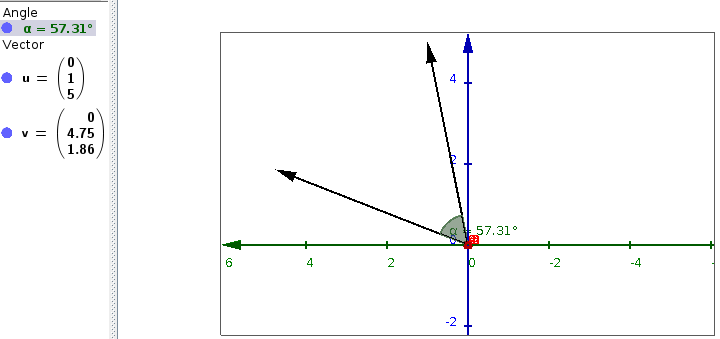
\includegraphics[width=12cm]{rotationsmatrix_eksempel.png}
  \caption{Eksempel på en rotationsmatrix}
  \label{fig:rotationsmatrix_eksempel}
\end{figure}
% Geogebra udregner vinkler i grader, så vi omregner grader til radianer ved hjælp af ligningen:
% \begin{equation}
  % R=d/2*\pi/360=57,31/2*\pi/360\approx1
% \end{equation}
Vi ser at vektor $\vv{u}$ blev drejet \theta radianer, som forventet.


\subsubsection{Fra 3D-model til billede}
I dette afsnit er det vist, hvordan der kan udledes en model, der beskriver en billeddannelsen af objekter i rummet, også kaldt rendering. Dette er essentielt da billeddannelsen danner grundlag for, hvordan 3D-modellen for en lampe omdannes til et billede, der kan vises for kunderne på e-butikken. Til sidst i afsnittet udledes en model for, hvordan belysningen fra en lampe kan simuleres og visualiseres vha. raytracing. 

\paragraph{Perspektiv projektion}
For at udlede en model for billeddannelsen, tages der udgangspunkt i en perspektiv projektion. Perspektiv projektion er en måde at danne et billede af 3D-objekter ved at projektere objekterne hen på et plan mod et kameraes position\cite{fig:perspective_projection}. Princippet bag perspektiv projektion er vist på figur \ref{fig:perspektiv_projektion}.

\begin{figure}[H]
  \label{fig:perspektiv_projektion}
  \centering
  \tdplotsetmaincoords{60}{130}
\begin{tikzpicture}[tdplot_main_coords]
\draw (0,0,0) -> (2,-8,2);
\path[fill=gray!30, draw=gray] (-2,-4,-2) -- (-2,-4,2) -- (2,-4,2) -- (2,-4,-2) -- (-2,-4,-2);
\draw (0,0,0) -- (1,-4,1);
\foreach \p in {(2,-8,2),(1,-4,1),(0,0,0)}{
	\draw plot [mark=*, mark size=2] coordinates{\p } ; 
	\node [above right] at \p {P};
}
\draw plot [mark=*, mark size=2] coordinates{(2,-8,2) } ; 
\draw plot [mark=*, mark size=2] coordinates{(1,-4,1) }; 
\draw plot [mark=*, mark size=2] coordinates{(0,0,0) }; 
\node [above right] at (2,-8,2) {P};
\node [above right] at (1,-4,1) {B};
\node [above right] at (0,0,0) {C};
\end{tikzpicture}
  \caption{Viser princippet bag perspektiv projektion af et punkt på et billedplan.}
\end{figure}



Som vist på figur \ref{fig:perspektiv_projektion} kan et punkt $P\in \mathbb{R}^3$ projekteres ned på billedplanen $\alpha$ ved at finde skæringspunktet $B$ mellem billedplanen $\alpha$ og en lysstråle $L$, som går fra punktet $P$ mod kameraets position $C$. Gør man nu dette for alle punkter på et objekt i rummet, og tegner skæringspunkterne på billedplanen, dannes et billede af objektet. Udfordringen er så at afgøre hvilken farve punkterne på billedplanen skal have, da dette afhænger af objektets egenskaber, samt hvilket udefrakommende lys der rammer objektet. 

For at løse denne udfordring, benytter vi i dette projekt raytracing, der som beskrevet under afsnit \ref{sec:computergrafik}, bygger på at simulere lysstrålers interaktion med forskellige objekter i rummet. Hvordan dette fungere er beskrevet i næste afsnit, hvor der er beskrevet en model for backwards raytracing.

\paragraph{Raytracing}
I modsætning til en perspektiv projektion af et punkt på et plan, er raytracing, hvor man i stedet for punktet i rummet, tager udgangspunkt i de lysstråler der danner billedet. Ved backwards raytracing følger man lysstrålerne baglæns og ser på, hvor stor en lysintensitet, den pågældende lysstråle har efter den har interageret med objekterne i rummet. Ud fra dette farves det tilhørende punkt på billedet, og på den måde kan man rendere et helt billede. På figur \ref{fig:raytracing_skitse} er det vist hvordan man kan konstruere en lysstråle ud fra et bestemt punkt på billedplanen, hvor lysstrålen er beskrevet ved en retningsvektor og et startpunkt.

\begin{figure}[H]
  \label{fig:raytracing_skitse}
  \centering
  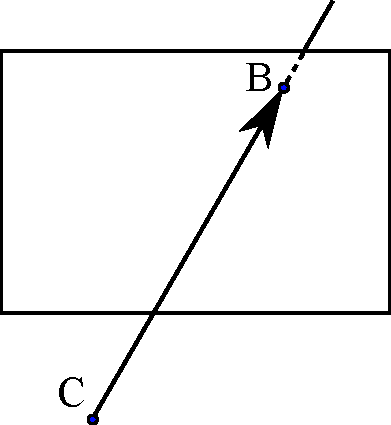
\includegraphics[width=5cm]{drawing}
  \caption{Viser hvordan en der kan opstilles retningsvektor mellem kameraets position $C$ og punktet $P$ på billedplanen, som sammen med startpunktet $C$ beskriver lysstrålen i omvendt retning.}
\end{figure}

Der findes flere forskellige modeller for hvordan lysintensiteten for en lysstråle beregnes. En simpel model, er Phong-modellen, som opdeler lys i forskellige kategorier: ambient, diffuse og specular.


\subsubsection*{Opsummering}

[Kort opsummerende beskrivelse af teorierne]

\subsection{Udvikling}

[Sammensætning af teorier igennem udviklingen af produktet, der løser problemet]

\subsection{Implementation}

Formålet med dette afsnit er at give en beskrivelse af programmets opbygning og struktur, samt ved brug af kodeeksempler at illustrere hvordan der gøres brug af den tidligere beskrevet teori til at lave programmet. I afsnittet vil der kun fremgå udvalgte kodeeksempler, men hele programmet kan findes i bilag. 

\subsubsection{Programbeskrivelse}

Programmet er udarbejdet som et suplement til hjemmesider som sælger lamper. Formålet med programmet er som beskrevet tidligere, at hjælpe kunderne med at visualisere lampers belysning. Programmet ligger fokus på realitsk visualisering af lys fra lamper, samt muligheden for at ændre pærens farvetemperatur.
Nedenstående figur viser et billede af renderingen fra det færdige program

#Indsæt rendering fra det færdige program

#nærmere beskrivelse af billede

\subsubsection{Programmets opbygning}

Programmet er opbygget efter desginprincippet "Top-down programmering". Princippet går ud på at dele programmet og i mindre dele, og derefter løse de mindre dele i hver deres funktion. Funktionerne samles i main, som kun bruges til kommunikation med brugeren. 




\clearpage

\section{Konklusion}
Formålet med dette afsnit er at opsummere hvordan den endelige problemformulering blev udarbejdet. Derudover konkluderes der hvorvidt den udviklede løsning besvarer den endelige problemformulering.

I problemanalysen, blev der argumenteret for det initierende problems relevans. I denne forbindelse blev der antaget at det initierende problem eksisterede, på baggrund af egne erfaringer, diskussion med lektor Lars Peter Jensen og en udtagelse fra en belysningskonsulent for en dansk lampebutik. Ønsket var at bekræfte antagelsen ved at udføre en spørgeskemaundersøgelse. Da denne undersøgelse aldrig blev fuldført, så er det ikke bevist, at det initierende problem eksisterer.
Efter argumentationen for problemets relevant blev begreber, interessenter og placering af det initierende problem undersøgt. Resultatet af disse undersøgelser dannede grundlaget for den endelige problemformulering.

Det første underspørgsmål i problemformuleringen var: \textit{"Hvordan visualiseres lyset fra en given indendørslampe?"}. Dette underspørgsmål blev besvaret ved at repræsentere lampen, som en 3D-model, som sammen med brugerinput om den ønskede visualisering, indlæses af programmet og renderes vha. raytracing med brug af phong-modellen beskrevet i afsnit \ref{sec:teori}.

Det andet underspørgsmål var: \textit{"Hvordan kan lampen og dens belysning visualiseres fra flere vinkler?"}. Dette underspørgsmålet blev besvaret ved at anvende teorien om rotationsmatricer i afsnit \ref{sec:teori}, til at positionere det virtuelle kamera, som billedet renderes ud fra.

Det tredje underspørgsmål var: \textit{"Hvordan visualiseres forskellige pærers lys?"}. Her blev der anvendt en algoritme, som konverterer en farvetemperatur for pæren til en RGB-værdi, som kunne benyttes i phong-modellen.

Problemformuleringens overordnede spørgsmål var \textit{Hvordan kan vi lave et værktøj til e-butikker, som visualiserer belysningen fra indendørslamper for kunderne?"}. Ud fra ovenstående kan det nu konkluderes, at problemformuleringen er delvist løst, da der er udviklet et værktøj, der kan visualisere en lampe og dens belysning med forskellige synsvinkler og farvetemperaturer. Problemformuleringen er kun delvist løst, da der stadigvæk er mangler i forhold til implementeringen af værktøjet på en e-butiks hjemmeside. Programmet mangler følgende:

\begin{itemize}
\item Bedre overenstemmelse af farvetemperaturen for pæren i den rigtige lampe i forhold farvetemperaturen på det renderede billede.
\item Lavere renderingstid for, at løsningen er praktisk anvendelig.
\item Brugerflade til visning af billeder.
\end{itemize}

\clearpage

\section{Perspektivering}
I dette afsnit forklares der hvad, der skal til for at arbejde videre på løsningen samt alternative anvendelsesmuligheder. 

For at arbejde videre på løsningen vil det være relevant at udvikle følgende:

\begin{itemize}
\item En brugerflade til visning af billeder på e-butiks hjemmeside.
\item Optimering af raytraceren, så renderingstiden formindskes. 
\item Viderudvikling af raytaceren med henblik på højere realisme.
\item Højere overenstemmelse med reel farvetemperatur for pærer.  
\item At lave en backend for kommunikationen mellem serveren, hvor billederne renderes samt en e-butiks hjemmeside.
\end{itemize}

Selvom løsningsforslaget i denne rapport er målrettet mod kunder, som handler lamper på en e-butiks hjemmeside, er der andre anvendelsesmuligheder for løsningsforslaget. Det kunne tænkes at løsningsforslaget også kunne visualisere lamper og deres belysning for kunder, der handler i en detailbutik ved at have en computer eller tablet, som har implementeret løsningen. 

I rapporten er det beskrevet, hvordan man kan konstruere et program, der renderer et billede på baggrund af en 3D-fil. Denne løsningsmodel kan nødvendigvis ikke kun bruges på lamper, men er også anvendelig til visualisering af andre produkter, som f.eks.\ elektronikprodukter, møbler mm.

\clearpage

\section{Appendiks}
\section*{Projektforslag}
\section*{IT og læring i folkeskolen}
Mange folkeskoler bruger i dag computeren i undervisningen. Hvordan kan man anvende computeren til at fremme indlæring i folkeskolen?

\subsection*{Problemstilling}
Folkeskolen er grundlaget for den videre uddannelse af den nye generation. Da mange folkeskoler anvender computere i undervisning, er det oplagt at undersøge hvordan der kan udvikles et værktøj til at styrke indlæringen i undervisningen ved brug af computere. \\
Hvordan udvikles et værktøj til computeren, der kombinerer IT og læring i folkeskolen?

\subsection*{Mål}
Målet er at udvikle et program, der kombinere IT og læring. Er der nogle problemer ved nuværende læringsværktøjer i folkeskolens undervisning, som kan løses ved hjælp af en datalogisk løsning?

\subsection*{Ekspempler på datalogiske problemstillinger}
Datastrukturer, algoritmer, udvikling af grafisk brugerflade (GUI).

\subsection*{Ekspempler på kontekstuelle problemstillinger}
Hvem er relevante at kontakte, når der skal udvikles et nyt læringsværktøj? Hvem skal læringsværktøjet udvikles til? Hvilke krav er der til et læringsværktøj? 


\subsection*{Forslagsstiller}
Gruppe B2-28 (SW1b2-28@student.aau.dk)
\clearpage

\section{Referencer}

\begin{thebibliography}{99}


\bibitem{kvalitativ_metode}
  Forklaring af kvalitativ metode,
  Den Store Danske.
  Set 25-11-2015.
  \url{http://www.denstoredanske.dk/Samfund,_jura_og_politik/Sociologi/Sociologisk_metodologi/kvalitative_metoder}

\bibitem{nummermetoden}
  Beskrivelse af nummermetoden, set 17-12-2015,
  \url{http://iva.ku.dk/refererkorrekt/tekshenvisninger/#Nummermetoden}

\bibitem{human_factors}
  Human Factors in Lighting, third edition,
  Peter R. Boyce, 2014.
  Sider 532-536.
  ISBN: 9781439874882.

\bibitem{ergonomi_arbejdsplads}
  Konsekvenser ved dårlig belysning på arbejdsplads mm.,
  ebscohost.
  Set 2-12-2015
  \url{http://web.b.ebscohost.com/ehost/detail/detail?sid=2898a5ec-e3ec-4bf2-b3b7-f4eb754cd767%40sessionmgr115&vid=0&hid=101&bdata=JnNpdGU9ZWhvc3QtbGl2ZQ%3d%3d#anchor=toc&db=buh&AN=7531667}

\bibitem{OSHA}
  Occupational Safety \& Health Administration,
  Set 16-12-2015.
  \url{https://www.osha.gov/}
  
\bibitem{CVS}
  Computer vision syndrom,
  gmj.
  Set 2-12-2015.
  \url{http://gmj.sljol.info/article/10.4038/gmj.v11i1.1115/galley/1023/download/}
  
\bibitem{ddo_visualisering}
  Definition af visualisering,
  Den danske ordbog.
  Set 27-10-2015.
  \url{http://ordnet.dk/ddo/ordbog?query=visualisere}
  
\bibitem{def_lys}
  Definition af lys,
  Videnskab dk.
  set 27-10-2015.
  \url{http://videnskab.dk/sporg-videnskaben/hvad-er-lys}
  
\bibitem{britannica_lys}
  Definition af lys,
  Britannica.
  Set 27-10-2015.
  \url{http://global.britannica.com/science/light}

\bibitem{integral_led}
  Om integral-led,
  integral-led.com.
  Set 2-11-2015.
  \url{http://www.integral-led.com/about-integral-led}
  
\bibitem{varm_kold}
  Definition af varm og kold lys,
  integral-LED.
  Set 27-10-2015.
  \url{http://www.integral-led.com/education/warm-white-or-cool-white}

\bibitem{american_heritage}
  American Heritage,
  The free dictionary.
  set 27-10-2015
  \url{http://www.thefreedictionary.com/lamp}

\bibitem{fysisk_kontra_online}
  The State of Retail 2015,
  Timetrade
  Sarah Wallace.
  Rapport udgivet i 2015.
  Side 22, figur 14.
  Copyright © 2015 by TimeTrade Systems, Inc.
  Set 3-11-2015.
  \url{http://www.timetrade.com/system/files/surveys/State_of_Retail_Report_Final_June15.pdf}

\bibitem{fortrydelsesret}
  Fortrydelse og returret,
  forbrug.dk.
  Set 28-10-2015.
  \url{http://www.forbrug.dk/Raad-og-rettigheder/Forbrugerleksikon/Fortrydelsesret}

\bibitem{ikea_returret}
  Ikeas returret,
  Ikea.
  Set 27-10-2015.
  \url{http://www.ikea.com/ms/da_DK/kundeservice/kundeservice_sporgsmaal_svar_kontakt_os.html?ICID=DKFOO_KONTAKT_230315}
  
\bibitem{ddo_ehandel}
  Definition af e-handel,
  Den Danske Ordbog.
  Set 26-10-2015.
  \url{http://ordnet.dk/ddo/ordbog?query=ehandel}

\bibitem{ddo_ebutik}
  Definition af e-butik,
  Den Danske Ordbog.
  Set 26-10-2015. 
  \url{http://ordnet.dk/ddo/ordbog?query=ebutik}

\bibitem{retsinformationen}
  Lov om forbrugeraftaler,
  Retsinformationen.
  Set 26-10-2015.
  \url{https://www.retsinformation.dk/forms/r0710.aspx?id=160666}

\bibitem{computergrafik_introduktion}
  A Short Introduction to Computer Graphics,
  Frédo Durand - MIT Laboratory for Computer Science.
  CSAIL.
  Set 5-11-2015.
  \url{http://people.csail.mit.edu/fredo/Depiction/1_Introduction/reviewGraphics.pdf}
  
\bibitem{Cylindo}
  Visual content and software as a service,
  Cylindo.
  Set 9-11-2015.
  \url{http://www.cylindo.com/}
  
\bibitem{rastarization} 
  Real-Time Massive Model Rendering, first edition, Sung-Eui Yoon, 2008. Side 31. ISBN: 9781598297928.

\bibitem{raytracing_for_begyndere}
  Ray Tracing: Graphics for the Masses, 
  Paul Rademacher of Department for Computer Science at the University of North Carolina at Chapel Hill.
  Department of Computer Science, University of North Carolina at Chapel Hill.
  Set 5-11-2015.
  \url{https://www.cs.unc.edu/~rademach/xroads-RT/RTarticle.html}

\bibitem{perspective_projection}
  Essential mathematics for games and interactive applications : a programmer's guide, second edition, James Van Verth \& Lars M   Bishop, 2008. Sider 212-236. ISBN: 9780080878614.
  
\bibitem{phong_paper}
  Illumination for computer generated pictures, Volume 18 Issue 6, Bui Tuong Phong \& Robert Ashenhurst, 1975. Sider 311-317. ISSN: 0001-0782.

\bibitem{stanford_phong}
  Raytracing, 
  CS148 AS3, Stanford University. 
  Set 01-12-2015.
  \url{http://graphics.stanford.edu/courses/cs148-10-summer/as3/instructions/as3.pdf}

\bibitem{tanner_helland}
  How to Convert Temperature (K) to RGB: Algorithm and   Sample Code,
  Tanner Helland.
  Set 04-12-2015.
  \url{http://www.tannerhelland.com/4435/convert-temperature-rgb-algorithm-code/}
  
\bibitem{charity_values}
  Blackbody color datafile, 
  Mitchell Charity. S
  et 04-12-2015.
  \url{http://www.vendian.org/mncharity/dir3/blackbody/UnstableURLs/bbr_color.htmle/}
  
\bibitem{tanner_helland_chart}
  Raw temperature vs RGB chart,
  Tanner Helland. 
  Set 09-12-2015.
  \url{http://www.tannerhelland.com/4435/convert-temperature-rgb-algorithm-code/raw_temperature_vs_rgb_chart/}

\bibitem{farvetemp}
  Beskrivelse af farvetemperatur, 
  Den Store Danske. 
  Set 13-12-2015.
  \url{http://www.denstoredanske.dk/It,_teknik_og_naturvidenskab/Elektricitet/Belysning/farvetemperatur}
  
\bibitem{solidworks}
  Liste af solidworks produkter, 
  solidworks. 
  Set 13-12-2015.
  \url{http://www.solidworks.com/sw/3d-cad-design-software.htm}

\bibitem{augmented_reality}
  Beskrivelse af augmented reality,
  Augmented Reality.
  Soha Maad
  Chapter 1, section 4
  ISBN 978-953-7619-69-5

\bibitem{artemides}
  Artemides Augmented Reality App, 
  Artemide.
  Set 14-12-2015.
  \url{http://www.artemide.com/blog/portfolio/the-new-version-of-artemide-augmented-reality-is-now-available/}

\bibitem{raytracingvsrastarizatioin}
  Fordele ved raytracing frem for rasterisering, set 16-12-2015,
  \url{http://www.tomshardware.com/reviews/ray-tracing-rasterization,2351-3.html}

\bibitem{softshadow}
  Beskrivelse af bløde skygger i raytracing, set 16-12-2015,
  \url{https://graphics.ethz.ch/teaching/former/seminar/handouts/Lang_SoftShadowVolumes.pdf}

\bibitem{rotationsmatricer}
  Weisstein, Eric W. "Rotation Matrix." From MathWorld--A Wolfram Web Resource, set 17-12-2015,
  \url{http://mathworld.wolfram.com/RotationMatrix.html}

%\bibitem{forbrugerportalen}
%  Definition af forbruger,
%  Forbrugerportalen
%  set 27-10-2015
  
%  \url{http://www.forbrugerportalen.dk/sider/artikel.asp?ID=13}


% \bibitem{prototyper_pdf}
%  Anvendelse af prototyper,
%  Teknologisk.dk
% set 27-10-2015
  
% \url{www.teknologisk.dk/_root/media/52285_Prototyping.pdf}

% \bibitem{fysiske_butikker}
% Forbrugere vil betale mere for varer i butikker,
% caltech.edu
% set 27-10-2015
  
% \url{http://www.caltech.edu/news/consumers-will-pay-more-goods-they-can-touch-caltech-researchers-say-1650}


% \bibitem{SolidWorks} 
%  3D CAD Software brugt af designere i IKEA,
%  set 17-11-2015
%  \url{http://www.3ds.com/products-services/solidworks/},
  
\end{thebibliography}
\clearpage

\section{Bilag}


\subsection{Mail fra lampedesigner Erik}
\label{sec:mailErik}
Kære Mathias

Det er en meget komplex opgave i der er igang med, der er mange faktorer i spil når det handler om lys, både de fysiske, men ikke mindst de mentale. Jeg har i en del år arbejdet med lampedesign. og har derfor mest været optaget af armaturets/lampens skulpturelle udtryk, men da det jo er en lampe skal den selvfølgelig  også opfylde det belysningsmæssige behov. Jeg har arbejdet med mange lyskilder, lige fra glødepæren til det nyeste LED.I alle mine lamper er valg af lyskilde og placering sket på grundlag af test via prototyper. de fleste af mine lamper er prototyper. En af de mest krævende lamper, har været Gedserlampen, der har et specielt designet armatur, der kan sammensættes til forskellige højder. Gedserlampen er en reflektorlampe, og lyskilden er LED. det krævede utallige målinger, og det foregik såmænd kl 12 om natten, en tommestok på jorden og et luxmeter. Jeg vil nok foretrække prototype test, da de jo er tæt på virkeligheden, men måske kunne jeres software være en god hjælp i den indledende fase af et projekt? Du er velkommen til at kontakte mig igen hvis du tror jeg kan bidrage med noget.

Held og Lykke med projektet.

Venlig hilsen

Erik Mortensen

\subsection{Mail fra lampedesigner David fra IKEA Sverige}
\label{sec:mailDavid}
Hi! Apart from hand sketching and physical prototypes, we use the 3D modeling application Solid Works in IKEA of Sweden. And for renderings we use either the built in renderer, or photo works, which is also part of solid works.

Regards 

//David 

  On 9 October 2015 15:19:41 +08:00, Lasse Fribo Gadegaard <lgadeg15@student.aau.dk> wrote:
   
  Hello
   
   
  We are seven students from Aalborg university, that are writing a project on lamps and how they are design. And so we would like to ask you if you use any software to visualize your design, before they are made as a prototype or finished product. If you use any software feel free to tell us so we could research the software and get a better insight in the industry. I really hope you can help us. Thanks
   
   
  Regards,
  7 Students from Aalborg university
  
\subsection{Mail fra belysningskonsulent}
\label{sec:mailbelysning}
Fra: XX \newline
Sendt: 6. november 2015 13:36 \newline
Til: Lasse Fribo Gadegaard\newline
Emne: SV: Semesterprojekt om lamper - AAU\newline
Hej
 
Det at se en lampe i 3D gør ikke at man ser lyset. Nogle af vores producenter laver allerede 3D modeller af deres lamper og endda sådan at man kan se lampen med lys i. Jeg har lige vedhæftet Artemides udgave af fremgangsmåden.

Men derfra til at se hvordan lyset er i et konkret rum hvor farver, højde mv. har indflydelse på lyset gør at det bliver en ekstrem kompleks størrelse der kræver komplicerede belysningsberegningsprogrammer som f.eks. DIALux. Lysberegning handler primært om lysmængde og ikke om lyseffekt.

Kunder har svært ved at forstå er hvilken lyseffekt lampen giver. Det er jo to-siddet. Dels vil de se hvordan lampen ser ud i rummet og dels vil de se hvordan lyseffekten er. Første del klarer flere producenter. Hvis man så bagefter at man har sat lampen ind som 3D model burde man lave et lag over billedet hvor producenten så har taget et billede af et rum hvor man kan se skygger mv. Eks Tom Dixon. Det er det jo ikke lampe man køber men ofte lyseffekt og lampe handler jo om at forme lyset og lave skygger. At sætte en Tom Dixon lampe ind i et rum gør ikke at du kan se skyggerne.

Det er blevet en kompliceret proces at producere en lampe ift. EU lovgivning i dag så jeg har svært ved at se at producenterne vil koste endnu flere penge til produkter til privatmarkedet som måske kun køber en lampe til 3000 kr. som ofte kun interesserer sig for den laveste pris og ikke den bedste service og rådgivning. Så producenters incitament til ligge investeringer hos privatkunder er meget begrænset. Mange laver end ikke et fritskravet billede af deres lampe. Og igen Tom Dixon anvender en klar halogenlyskilde. Hvis du sætter en klar kultrådslyskilde hvor filamentet er længere giver forsat skygger men på en blødere måde da lyset er delt ud på en større overflade. Hvis du sætter en mat lyskilde i forsvinder skyggerne næsten helt. Pludselig er løsningen bare komplekst og når en producent så har 4000 varenumre. Samme lyskilder laves så i 3 farvetemperaturer. Med vores adgang til varesortiment giver det 2 mio. billeder dokumenter som skal indhentes. Så er vi der hvor det begynder ikke at hænge sammen tidsmæssigt når nethandlen handler om at være først ift. googlesøgninger mv. Hvem har lyst til at give bedste rådgivning ift. lyseffekter hvis man ender på side 20 når folk søger på google?  

Løsningsforslag modtages derfor med kyshånd da kompleksitet er desværre nem at se. 

I må selvfølgelig også gerne vores udtagelser.  

Med venlig hilsen / best regards

XX\newline
Belysninskonsulent

\noindent\makebox[\linewidth]{\rule{\paperwidth}{0.4pt}}

Fra: Lasse Fribo Gadegaard [mailto:lgadeg15@student.aau.dk] \newline
Sendt: 6. november 2015 11:19\newline
Til: XX\newline
Emne: SV: Semesterprojekt om lamper - AAU

Hej 
 
Vi er meget glade for at I vil bidrage til projektet. Indtil videre har vi analyseret problemet: 
Forbrugeren kan ikke visualisere, hvordan lyset udbreder sig fra en lampe uden at købe og installere lampen. 

I problemanalysen har vi undersøgt interessenter, begreber, placering og teknologier til problemet. 

Ud fra dette har vi valgt at fokusere på e-butikker, der sælger indendørs lamper til brug i erhverv eller private hjem. 

Vi har netop udarbejdet den endelige problemformulering, hvor udkastet lyder som følgende:
Hvordan kan man lave et værktøj til e-butikker som vha. raytracing*, visualiserer belysningen fra indendørs lamper for kunderne? 

* En teknik til at simulere lys og lave et billede af en 3D-model. 

Vi skal nu til at udvikle en løsning til problemet, og hertil har vi lavet en simpel skitse (Se vedlagt billede) af den ide vi har på nuværende tidspunkt. 
 
Som vist på skitsen, er ideen at lave et produkt som gør det muligt for kunderne at se nogle lamper og deres belysning i et interaktivt 3D-billede på e-butikken. 

Vi tænker at forbrugeren skal kunne gøre følgende: \newline
 - Vende og dreje billede, så de kan se lampen og belysningen fra flere vinkler. \newline
 - Se lampen med forskellige pærer (evt. angive farvetemperatur i Kelvin) \newline
 - Skifte den kontekst som lampen visualiseres i (f.eks. forskellige rum/møbler)

Pga. tidsbegrænsning forventer vi ikke at lave hele løsning, som produkt, men blot implementere de mest studierelevante dele. 

Dog skal vi stadigvæk præsenterer en færdig løsning i rapporten. 

Det vi nu ønsker jeres respons på, er følgende
 - Jeres tanker omkring ideen, som løsning på problemet.\newline
 - Forslag og ønsker til forbedringer af ideen. \newline
 - Jeres accept til, at vi i rapporten må inddrage jeres udtagelser anonymt.

Med venlig hilsen,\newline
Lasse Gadegaard
 
På vegne af \newline
Gruppe B2-28\newline
Software, AAU
 
\noindent\makebox[\linewidth]{\rule{\paperwidth}{0.4pt}}

Fra: XX \newline
Sendt: 5. november 2015 15:43\newline
Til: Lasse Fribo Gadegaard\newline
Emne: SV: Semesterprojekt om lamper - AAU\newline
Hej Lasse

Det lyder til at være et meget spændende projekt.
 
Som primær detailforretning med projektafdeling lever vi af konsulentarbejde ved at give rådgivning omkring hvordan lys forandre sig ift. til lofthøjde, farver, armatur, lyskilde foruden at der er en subjektiv mening om hvad godt lys er.

Der er overraskende mange der gerne vil se lyset inden de køber lamper. Man kan dog undre sig ovre at samme kunde køber både køleskabe, vaskemaskiner mv. uden at stille krav til at prøve tingene før de køber varerne selv om disse produkter koster lige så meget som de lamper vi sælger. Kunder har åbenbart et specielt forhold til lys. 

Har i allerede valgt teori, metode og empiri? 

Jeg tror godt vi kan hjælpe jer. Eneste krav er at data herfra bliver anonymiseret og vi får et eksemplar af opgaven når den er skrevet.

God dag

Med venlig hilsen / best regards\newline
XX\newline
Belysningskonsulent

\noindent\makebox[\linewidth]{\rule{\paperwidth}{0.4pt}}

Fra: Lasse Fribo Gadegaard [mailto:lgadeg15@student.aau.dk] \newline
Sendt: 5. november 2015 15:06\newline
Til: XX\newline
Emne: Semesterprojekt om lamper - AAU
 
Hej XX
 
Vi er en gruppe på Aalborg Universitet, som er i gang med et projekt om visualisering af lamper.
 
Vi arbejder med følgende problemstilling:
"Forbrugeren kan ikke visualisere, hvordan lyset udbreder sig fra en lampe uden at købe og installere lampen." 

Vi har fokus på e-handel, og ønsker at tilbyde e-butikken et værktøj som gør det nemmere for kunderne at visualisere, hvordan lyset breder sig ud fra en lampe (f.eks. hvilke skygger, mønstre og farver som lampen udsender). 

Derfor søger vi nu e-butikker, som ønsker at bidrage med viden og informationer omkring e-handel med lamper.  

Hvis I er interesserede i at medvirke i projektet, så skriv venligst tilbage på mail: lgadeg15@student.aau.dk 

Med venlig hilsen,\newline
Lasse Gadegaard\newline
På vegne af\newline
Gruppe B2-28\newline
AAU, Software

%clearpage for at CD er på egen side
\clearpage
\subsection{CD}

Vedlagt på CD-rom:

\begin{itemize}
  \item Program.zip
  \item Rapport.pdf
  \item Billeder af tests
\end{itemize}



%clearpage for at få projektforslag på egen side
\clearpage
\subsection{Projektforslag}

\section*{INDSÆT EMNE}

indledning til emne

\subsection*{Problemstilling}

\subsection*{Mål}

\subsection*{Ekspempler på datalogiske problemstillinger}

\subsection*{Ekspempler på kontekstuelle problemstillinger}

\subsection*{Forslagsstiller}

Gruppe B2-28 (SW1b2-28@student.aau.dk)

\clearpage




\end{document}
